%%%%%%%%%%%%%%%%%%%% author.tex %%%%%%%%%%%%%%%%%%%%%%%%%%%%%%%%%%%
%
% sample root file for your "contribution" to a contributed volume
%
% Use this file as a template for your own input.
%
%%%%%%%%%%%%%%%% Springer %%%%%%%%%%%%%%%%%%%%%%%%%%%%%%%%%%%%%%%%%


%% RECOMMENDED %%%%%%%%%%%%%%%%%%%%%%%%%%%%%%%%%%%%%%%%%%%%%%%%%%%
%\documentclass[graybox]{svmult}
%
%% choose options for [] as required from the list
%% in the Reference Guide
%
%\usepackage{mathptmx}       % selects Times Roman as basic font
%\usepackage{helvet}         % selects Helvetica as sans-serif font
%\usepackage{courier}        % selects Courier as typewriter font
%\usepackage{type1cm}        % activate if the above 3 fonts are
                             % not available on your system
%
%\usepackage{makeidx}         % allows index generation
%\usepackage{graphicx}        % standard LaTeX graphics tool
%                             % when including figure files
%\usepackage{multicol}        % used for the two-column index
%\usepackage[bottom]{footmisc}% places footnotes at page bottom
%
%% see the list of further useful packages
%% in the Reference Guide
%
%\makeindex             % used for the subject index
%                       % please use the style svind.ist with
%                       % your makeindex program
%
%%%%%%%%%%%%%%%%%%%%%%%%%%%%%%%%%%%%%%%%%%%%%%%%%%%%%%%%%%%%%%%%%%%%%%%%%%%%%%%%%%%%%%%%%%
%
%\begin{document}

\title{Artificial Intelligence and Machine Learning}
% Use \titlerunning{Short Title} for an abbreviated version of
% your contribution title if the original one is too long
\author{
    \textbf{Kincho H. Law}
    \and {Barbaros Cetiner}
    \and {Sascha Hornauer}
    \and {Frank McKenna}
    \and {Satish Rao}
    \and {Ertugrul Taciroglu}
    \and {Chaofeng Wang}
    \and {Qian Yu}
    \and {Stella Yu}}
\tocauthor{}
\authorrunning{Law et al.}
% Use \authorrunning{Short Title} for an abbreviated version of
% your contribution title if the original one is too long
%\institute{Name of First Author \at Name, Address of Institute, %\email{name@email.address}
%\and Name of Second Author \at Name, Address of Institute %\email{name@email.address}}
%
% Use the package "url.sty" to avoid
% problems with special characters
% used in your e-mail or web address
%
\maketitle

At present, Artificial Intelligence and Machine Learning (AI/ML) research is one of the fastest-growing fields in academia and industry. Between 1998 and 2018, the volume of peer-reviewed AI papers has grown by more than 300\%, accounting for 3\% of peer-reviewed journal publications and 9\% of published conference papers \citep{perrault2019ai}. The global market for machine learning technologies, including hardware, software and services, is expected to grow astronomically from about \$3 Billion in 2017 and the current \$7 Billion in 2020 to over \$30 Billion in 2024 (Market Research Future, 2019). AI/ML technologies have already penetrated in many aspects of our everyday life, including health care, business and commerce, transportation, agriculture, manufacturing, natural and built environment, education, etc.. They will continue to have tremendous impacts to our society as a whole (National Science and Technology Council, 2016a, 2016b, 2019). As advances in computing technologies such as computer graphics, finite element methods and CAD/CAE have had in the past, AI/ML will potentially revolutionize how engineering modeling, design, and simulations are conducted. With rapid advances in hardware and software technologies, and continuing developments in all aspects of computational science and engineering, natural hazards engineering and simulations will be dramatically impacted by AI/ML.

Generally speaking, the field of artificial intelligence (AI) aims to create computational systems (or machines) that behave and solve problems in ways that emulate human intelligence. Often based on stipulated rules and pieces of knowledge, AI systems have the ability to learn, reason, adapt to changes, and self-correct with facts and data. Machine learning (ML) is a sub-field of AI that enables machines to learn from past data or experiences, self-adapt in a changing environment, and self-correct with new information. By optimizing the (feature) parameters of an ML model using training data or past experiences, the model may have the ability to make generalizations and predictions for certain events in the future and/or gain new knowledge within the model domain. Deep learning (DL), typically consisting of many (deep) layers of computational units, is a technique for realizing machine learning by automatically discovering possible model features from the data. Data mining shares many of the same techniques in machine learning. However, data mining aims to discover interesting patterns, extract rules, or construct models from large volumes of data. While data mining models possess high predictive ability similar to ML models, they often lack the "intelligence" to learn and adapt automatically to changes. As opposed to optimization, where a single well-defined objective function of the problem is to be maximized or minimized, a machine learning model is devised from the training data by finding the optimal values for the (feature) parameters using scoring metrics that give the best predictive accuracy. While a mathematically optimized model is not easily adapted to a new set of parameters, constraints, or data, a machine learning model may be generalized to apply beyond the training data; the model can be adapted and transferred—with appropriate accuracy measurements and validation—to build models for problems of similar types. 

The purpose of this report is to provide a brief review of the latest AI/ML technologies and how they can potentially be applied to natural hazards engineering (NHE). As AI/ML is a rapidly growing field with new methods and new applications being discovered constantly, comprehensive coverage of all the developments is beyond this report's scope. The report is purposely written in general terms with a short introduction to the different methodologies in AI and machine learning. Similarly, NHE is a very broad field dealing with impacts due to earthquake, tsunami, wind/hurricane, flood, liquefaction, fire, and other hazards. Covering all possible applications of AI/ML in all hazard areas is a task beyond this report and the ability of the writers. A few selected examples of prior works in different natural hazard domains are briefly described herein to illustrate the potential applications of AI/ML. Additionally, some of the ongoing efforts on the use of deep learning methods at the SimCenter towards the development of workflows for natural hazard modeling and analysis are discussed. Lastly, potential opportunities for AI/ML technologies in NHE are discussed to engender further research and developments in this field. Finally, it should be emphasized that the references and the works cited in this report represent only a small number of illustrative examples in the field as the possibilities of AI/ML are almost boundless. 

\section{Overview of AI/ML methods}
\label{sec:ai_methods}

\noindent\textbf{Knowledge-Based Expert Systems} \\Since the 1950s, when the term Artificial Intelligence (AI) was coined, considerable progress has been made. Early research and developments in the 1980s (often known as the first wave of AI) was dominated by the rise of rule-based expert system and knowledge-based expert system (KBES) technologies (Haye-Roth et al., 1983). With expert knowledge handcrafted as "if-then" or logic rules, expert systems with enabled reasoning and inference mechanisms have been used to address many interesting ill-posed problems, albeit often in some narrowly defined domains (Simon, 1973). One class of ill-posed problems arise is the conceptual structural design of buildings which often requires prior experiential knowledge and considers downstream design and construction constraints (Sriram, 1985; kumar1997cadrem; Jain et al., 1991a, 1991b). Indeed, KBES technologies have created significant excitement in all disciplines of civil engineering, —including structural, geotechnical, earthquake, transportation, and environmental engineering (Kostem and Maher, 1986, Palmer, 1987; dym1991knowledgebased; cohn1992knowledgebased; Sriram, 1997). How knowledge is represented is crucial to the usefulness of KBES as the representation would dictate how the system interacts with rules and data. While research on KBES has slowed down for the past couple of decades, advances in semantic information modeling and ontology continue to prevail (Stevens et al., 2000,noy2009bioportal}. For instance, in civil engineering, research on semantic modeling and the process of capturing the semantic information about buildings and infrastructures has given rise to Building Information Modeling, which has been embraced by the building and construction industry worldwide for the delivery of project information throughout a facility lifecycle \citep{sacks2018bim}. Ontology, with defined terms and relationships among the terms in a domain, can play a critical role in bringing together disparate sources of information and effectively supporting NHE modeling and simulation, for example, in estimating earthquake damages to structures and infrastructures \citep{yu2016image}.
\newline
 
\noindent\textbf{Statistical-Based AI} \\AI research and developments in the 1980s and 1990s have also brought popularity for a number of reasoning and inference mechanisms (such as decision trees, Bayesian networks, etc.) and statistics-based classification, clustering and regression techniques (such as logistic regression, k-means, random forest, etc.) that find ample applications in data mining and knowledge discovery as well as in engineering. For instance, Bayesian networks are commonly used in structural reliability analysis (Straub and Der Kiureghian, 2010). Boosted decision trees have been applied to detect pipe failures and to assess weak points of geographically distributed water systems (Winkler et al., 2018,kumar2018using}. Neural networks (also commonly known as artificial neural networks, or ANNs) have emerged as a powerful computational and knowledge representation paradigm to build self-organized models that are able to discover patterns or draw associative relationships between input and output data \citep{bishop1995neural}. Fitting (mathematical) models to experimental data and extracting knowledge from the data to explain physical observations are nothing new in science and engineering. However, the ability for a computational "machine" to automatically "learn" models by analyzing the data and extract relationships and patterns can have important implications for modeling complex systems. Neural networks have found many applications in all disciplines of civil engineering (Garrett and Smith, 1996,kartam1997artificial}. For instance, instead of expressing material behaviors and constitutive relations in mathematical forms, neural network models are trained to represent constitutive models and thermal properties of complex materials, such as composites and laminated materials, and nonlinear behaviors of structural components directly using experimental data and observations (Ghaboussi et al., 1991; ghaboussi1998autoprogressive; aquino2006self). 
\newline
 
\noindent\textbf{Kernel-Based Methods} \\Another notable development in data-driven machine learning is a class of statistical-based Kernel methods (such as support vector machine (SVM), principal component analysis (PCA), Gaussian process regression (GPR) models), that draw on measuring similarity between data samples (Rasmussen and Williams, 2006,hofmann2008kernel}. Like neural networks, kernel methods, such as support vector regression (SVR), have been employed to develop material and component behavior models (see, for example, luo2018machine). Kernel methods are also commonly used as surrogate models in multiscale modeling, inverse problems, and optimization (Wirtz et al., 2012; Park and Law, 2016; eriksson2018scalable; Santin and Haasdonk, 2019). Often known as Kriging in geoscience and mapping, kernel methods have been widely used for geospatial analysis and employed as geostatistical estimator for interpolating geospatial information with quantifiable uncertainties (Olea, 2012,jia2016surrogate}. As material modeling, multiscale modeling and analysis, inverse and optimization problems, reliability analysis and uncertainty quantifications, regional geostatistical analysis are all fundamental components of NHE, AI-based inference, and statistical and data-driven machine learning methods are likely to find ample applications in natural hazards modeling and simulation. 
\newline

\noindent\textbf{Deep (Machine) Learning} \\With the present abundance of data of different types (text, time series, numerical/audio/video data, images, etc.) available from a large variety of sources (web and social media) as well as devices (sensors, cameras), data-driven statistical learning (often known as the second wave of AI) has become popular since the 2000s; and this area of research has largely been dominated by the so-called deep learning (DL) \citep{lecun2015deep}. DL methods are typically based on multi-layered neural networks that can automatically discover features from the data and use the learned features to perform prediction and make decisions for a specific task. Many different deep learning architectures exist—such as deep (multi-layered) neural networks, recurrent neural networks, convolutional neural networks, generative adversarial networks, and many others—, with each having different designs and learning strategies. The learning or training process can be typically classified by supervised (with labeled training data), unsupervised (without labeled training data), semi-supervised (with a small number of labeled but large amounts of unlabeled data), or iterative reinforcements (by optimizing the model according to some pre-defined criteria and policy). Deep learning methods have been successfully applied to many fields, such as computer vision, image processing, speech and audio recognition, natural language processing and language translation, and produce results that often exceed human expert performance. The successes of DL, particularly in pattern recognition and computer vision, have drawn significant attention in the civil and environmental engineering community. Within structural engineering, deep learning methods have been widely applied in the field of structural health monitoring (Salehia and Burguenoa 2018). By treating the damage detection problem as object detection, and classification and segmentation of images, computer vision (CV) based DL methods have been applied successfully detect and identify many types of structural and material damages (cha2017deep; ferguson2018detection; Gao and Mosalam, 2018a,yeum2019automated,enjani2020automated}. For instance, during the 2018 Structural ImageNet and PEER Hub ImageNet Challenge (Gao and Mosalam, 2018b), DL methods are shown capable of performing relatively well on several detection tasks, including classification and identification of scenes, damage states/levels/types, material types, collapse states, and component types. With the publicly available street and satellite images, CV-based DL methods hold significant potential for being an integral component in (regional) natural hazards modeling and simulations.

Among these approaches, knowledge-based expert systems are intuitive and interpretable, but building them requires a lot of domain knowledge. In contrast, statistics-based AI and kernel-based methods are more data-driven, often requiring handcrafted features. The former approach assumes that the features are given, while the latter finds ways to implicitly lift the given feature to a more expressive space. The significance of deep learning approaches is that it eliminates the need for feature engineering and allows a classification or regression model to be trained entirely from the data in an end-to-end learning fashion. With the availability of large-scale data sets and increasingly powerful computing hardware such as GPUs, DL models that have a very large numbers of parameters can be explored and—particularly for problems that are highly "nonlinear" in nature—can deliver high performance unmatched by previous approaches.

\section{AI/ML in Natural Hazards Engineering}
\label{sec:ai_nathaz}

AI/ML has been applied across many fields of natural hazards engineering (NHE) for quite some time and has gained increasing popularity in recent years. Such applications range from data acquisition, hazard modeling, engineering simulation, reconnaissance studies, to developing predictive surrogate models using observed and simulated data. The following are some examples of machine learning applications in the areas of natural hazards.

\begin{itemize}
 \item In earthquake engineering, ML has been used for seismic wave discrimination and early earthquake warning \citep{li2018machine}, ground motion simulation \citep{alimoradi2015machinelearning}, pre-earthquake vulnerability screening \citep{yu2019building}, post-earthquake damage detection from imagery data \citep{cooner2016detection,bai2017machine}, and seismic damage and risk analysis of structures \citep{gidaris2015kriging}. Deep‐learning approaches have also been shown capable of estimating earthquake magnitude from recorded raw seismic signals \citep{mousavi2020machine}. Recently, a comprehensive review of the current and potential applications of AI/ML to a broad range of research in earthquake engineering has been provided by \citet{xie2020promise}. 
 \item Landslides, induced by earthquakes or heavy rainfall, are another natural hazard phenomenon that has attracted much attention \citep{dou2014gisbased}. Machine learning methods such as SVM, ANN, Kriging, Random Forest, etc., have been employed to predict the susceptibility of a landslide based on topographic, geological, and hydrological data \citep{yao2008landslide,goetz2015evaluating,pham2016comparative}. More recently, deep convolutional neural networks have shown the potential for recognizing landslides using aerial and satellite imagery \citep{ghorbanzadeh2019evaluation}.
 \item Flood is one of the most destructive natural hazards, which can cause massive damage to the built infrastructural systems and significant socioeconomic loss. ML methods have been shown to provide better insight for flood prediction and better predictive accuracy that outperform conventional modeling approaches (abbot2014input,mosavi2018flood}. Methods such as ANN, SVM, SVR, long short-term memory (LSTM), neuro-fuzzy, decision tree, etc., have been found effective for short- or long-term flood susceptibility and damage assessment (kim2016realtime,gizaw2016regional,resch2018combining,arabi2019urban,e2019application}. More recently, deep convolutional neural networks have been employed for regional flood susceptibility analysis using remote sensing images (gebrehiwot2019deep; li2019urban; Wang and Fang et al., 2020). 
 \item Hurricanes are another disastrous hazard that can cause significant damage to buildings and infrastructure systems. It has been shown that ML methods such as ensemble learning and bagging decision trees are capable of predicting wind-induced damages of individual buildings with better accuracy compared to HAZUS models \citep{subramanian2013constructing}. Methods such as random forest and logistic regression have also been employed to predict damages to residential structures due to hurricanes and high winds (Salazar, 2015). Deep learning has been applied to classify damages using post-hurricane aerial imagery (Thomas et al., 2011; Li and Ye et al., 2018; kersbergen2018automated). 
\end{itemize}

The examples cited are merely illustrative examples of a wide range of possible applications of AI/ML to NHE, from hazards susceptibility analyses to post-disaster renaissance studies. Complementary to conventional numerical modeling and simulations, AI/ML can be employed to support a number of NHE tasks, such as characterization of the built, natural, and socioeconomic environments, enhancing understanding of hazard models, constructing data-driven response estimation models, assessing structural performance, and simulating recovery processes. Among the many challenges in applying data-driven AI/ML methods to NHE is the critical need in gathering, generating, and managing the data, as well as making the data readily usable for NHE modeling and simulations \citep{padgett2020workshop}

\section{SimCenter's Ongoing AI/ML Efforts}
\label{sec:ai_simcenter}

As noted, significant research efforts have been reported in applying ML methods to natural hazards engineering. With the advances in computer hardware and the abundance of data, in the form of text, time-series signals, point clouds, and images that are being generated and made publicly available (Rathje et al. 2017), innovative applications of advanced ML technologies in natural hazard engineering will undoubtedly continue to grow. Nevertheless, extracting meaningful information from such data and rendering the data useful for natural hazard modeling and simulations is labor-intensive and computationally demanding and requires significant infrastructural investments. Another challenge is that data from public sources is often incomplete with missing information. Learning from available data, ML can potentially and effectively extract the relevant features and reconstruct the missing information, which are needed for engineering analyses and hazard modeling. As shown in Figure \ref{fig:AI_NHE_Computational_Framework}, one of the ongoing efforts at the SimCenter is to develop frameworks for natural hazards modeling and simulation and to demonstrate the workflows from data acquisition to hazard/risk analyses and simulation. Machine learning can play a key role in the overall workflows for NHE modeling and analysis, particularly for regional-based simulations. 

\begin{figure}[htb]
    \centering
    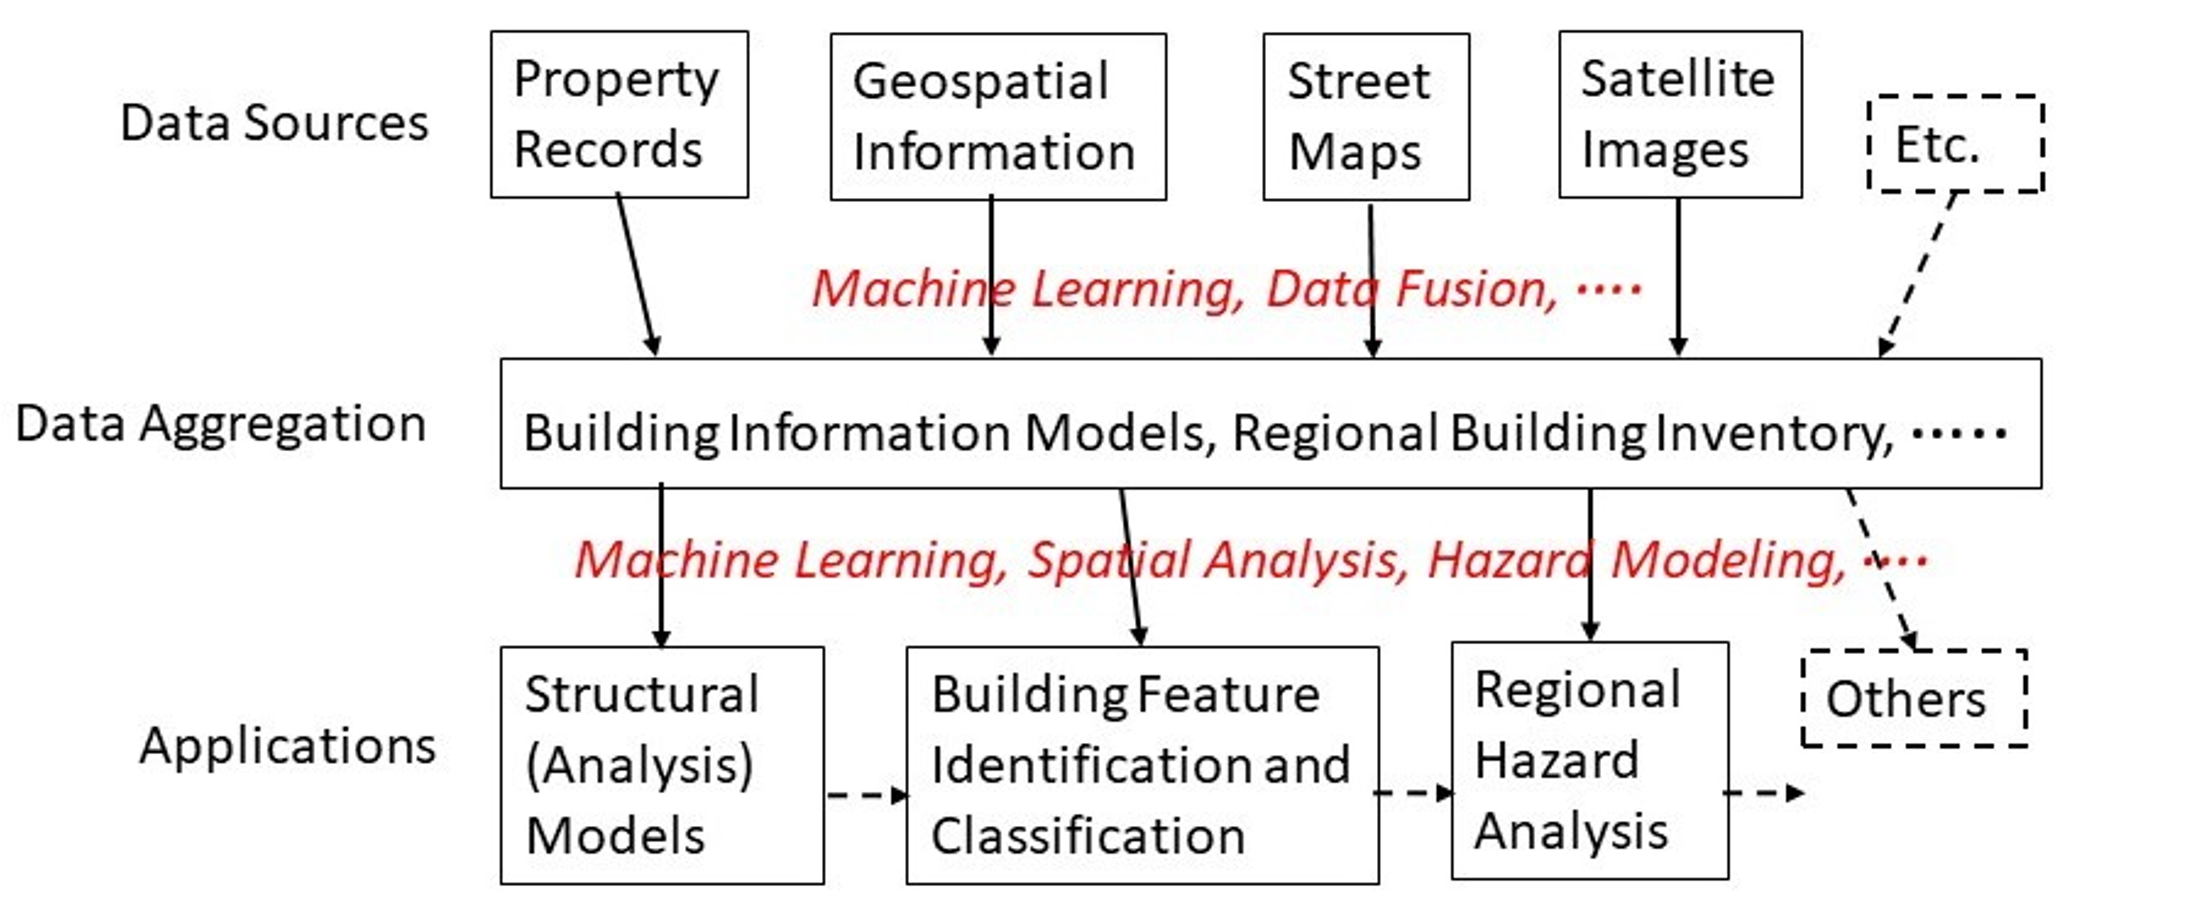
\includegraphics[width=1.0\textwidth, angle = 0]{Figures/AI_NHE_Computational_Framework.png}
    \caption{Computational Framework for Natural Hazards Modeling and Analysis – From Data Acquisition to Simulations}
    \label{fig:AI_NHE_Computational_Framework}
\end{figure}

\subsection{From Building Information Model (BIM) to Structural Analysis Model (SAM)}

Widely adopted by the architecture, engineering, and construction professionals, building information modeling is defined as a process that involves the generation and management of a "shared digital representation of physical and functional characteristics of any built object [...] which forms a reliable basis for decisions" (ISO, 2016). The digital Building Information Models (BIMs) can be an ideal source of information for natural hazard analyses. For example, based on the data and information captured in a BIM, structural analysis models (SAM) can potentially be created for dynamic finite element analysis of buildings under seismic or wind load conditions \citep{lu2020cimpowered}. 

Converting BIM to SAM, however, is not a trivial process and requires advanced knowledge of computer-aided design, structural engineering, finite element method, and practical experience. Manual conversion is an expensive and labor-intensive task, especially for large-scale regional simulation. To this end, SimCenter has initiated an effort to develop a framework to demonstrate the applicability of ML for bridging the gap between building information model (BIM) and structural analysis model (SAM).

The BIM-to-SAM framework is schematically shown in Figure \ref{fig:BIM_to_SAM}. Information in BIM is first distilled into a vector representing the features of the BIM. These features are then used as the input to a neural network, which yields another vector that represents features of the corresponding SAM. Based on the generated features, a SAM can be constructed programmatically. The BIM and SAM can then be stored in a standard neutral file format, such as JSON, which is a data-interchange format that uses human-readable text to store and transmit data objects consisting of attribute-value pairs and array data types. It should be emphasized that the framework is designed primarily to illustrate the overall workflow and the tasks involved in generating SAM from BIM using the ML approach. Continuing research and development efforts are needed to generalize the methodology, from the current experimentation on modeling of structural walls and frames to other structural components and systems. Demonstrations of the framework can be found in SimCenter's GitHub repositories (Wang and Jiang et al., 2019; Wang and McKenna, 2019).

\begin{figure}[htb]
    \centering
    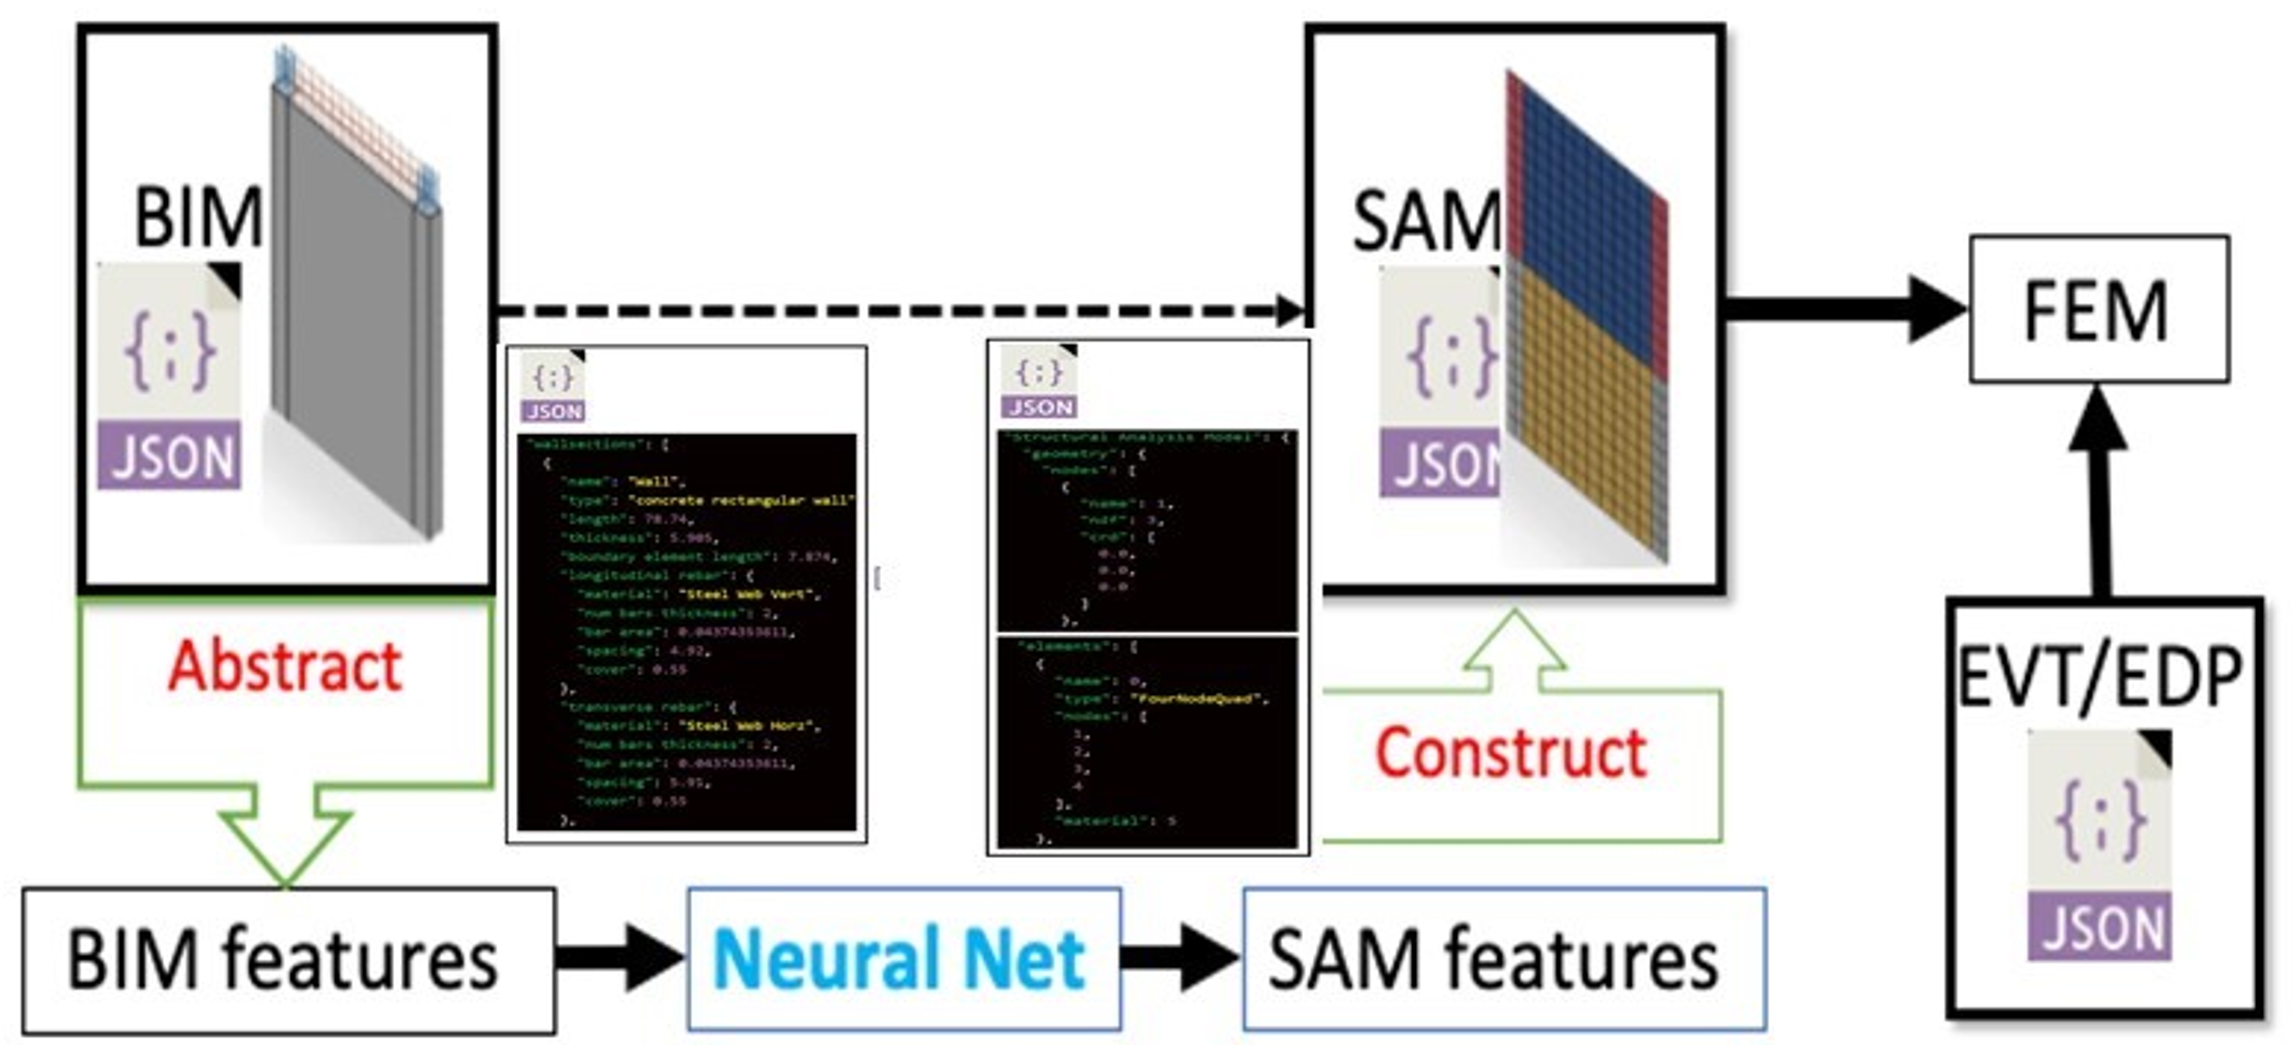
\includegraphics[width=1.0\textwidth, angle = 0]{Figures/BIM_to_SAM.png}
    \caption{BIM to SAM framework}
    \label{fig:BIM_to_SAM}
\end{figure}

\subsection{Building Features Extraction and Characterization—Soft Story Identification}

Rapid and accurate identification of building features and structural integrity is crucial in evaluating the seismic vulnerability of buildings city-wide. Structural irregularities due to abrupt variations of story stiffness, such as a soft-story building, increase the likelihood of damage to a building during a moderate or severe earthquake. Identifying and retrofitting soft-story buildings in a city represents a vital effort in earthquake preparedness and mitigation. However, soft-story building identification at a city-scale is a labor-intensive and time-consuming process. Visual screening is often the first step in the identification process. For instance, FEMA 154 (atc2015handbook) provides a screening methodology to evaluate the seismic safety of buildings mainly based on the visual cues of the building exteriors and to determine whether a building requires more detailed evaluation. The purpose of this effort is to design a workflow that can be applied to rapidly identify potential soft-story buildings on a city scale. 

The availability of street-view images and recent advances in computer vision and machine learning techniques make the automated screening of soft-story buildings a viable proposition. Structural attributes—e.g., frame types, geometric irregularities, and foundation conditions—can often be identified from certain observable visual cues. Many of such visual cues—such as a garage with relatively narrow wall widths on both sides of the garage opening, large opening at the ground floor level, a story with less wall area or fewer columns than other stories, etc.—are used by trained professionals to rapidly screen for potential soft-story buildings. However, the visual screening process remains labor-intensive, as it requires collecting a large amount of image data on the buildings, and subjective interpretations can be error-prone. An automated process that is able to extract building features and identify a specific type of structural vulnerability by interpreting the relevant features can be beneficial to the rapid screening of a large number of buildings in a city or a region. 

As a demonstrative workflow on visual screening of building features, the SimCenter has developed an automated process using a machine learning approach to rapidly identify buildings that potentially have soft-story characteristics (Yu et al., 2019,yu2020building}. Using the data available for the study, five cities in California, namely Santa Monica, Oakland, San Francisco, San Jose, and Berkeley, are selected. As shown in Figure \ref{fig:soft_story_identification}, the first step of the workflow process is to collect street view images of the buildings (for example, using Google Street View Static API) based on the addresses in each city obtained from the official city website. A training set is then developed with annotations to train the soft-story classification model using convolutional neural networks, such as the Inception \citep{szegedy2016rethinking,szegedy2017inceptionv4} and ResNet \citep{he2016deep} architectures. The trained classification model can then be used to identify potential soft-story buildings in the city of interest. Two specific novelties of the workflow are worth mentioning. First, as a large number of images need to be labeled as having a soft-story or not, a semi-automated annotation process has been developed to minimize the manual labeling effort. Second, as shown in Figure \ref{fig:soft_story_identification}, a class activation map \citep{zhou2016} is employed to highlight the regions (that are likely corresponding to soft-story) and to help interpret the predictive results.

\begin{figure}[htb]
    \centering
    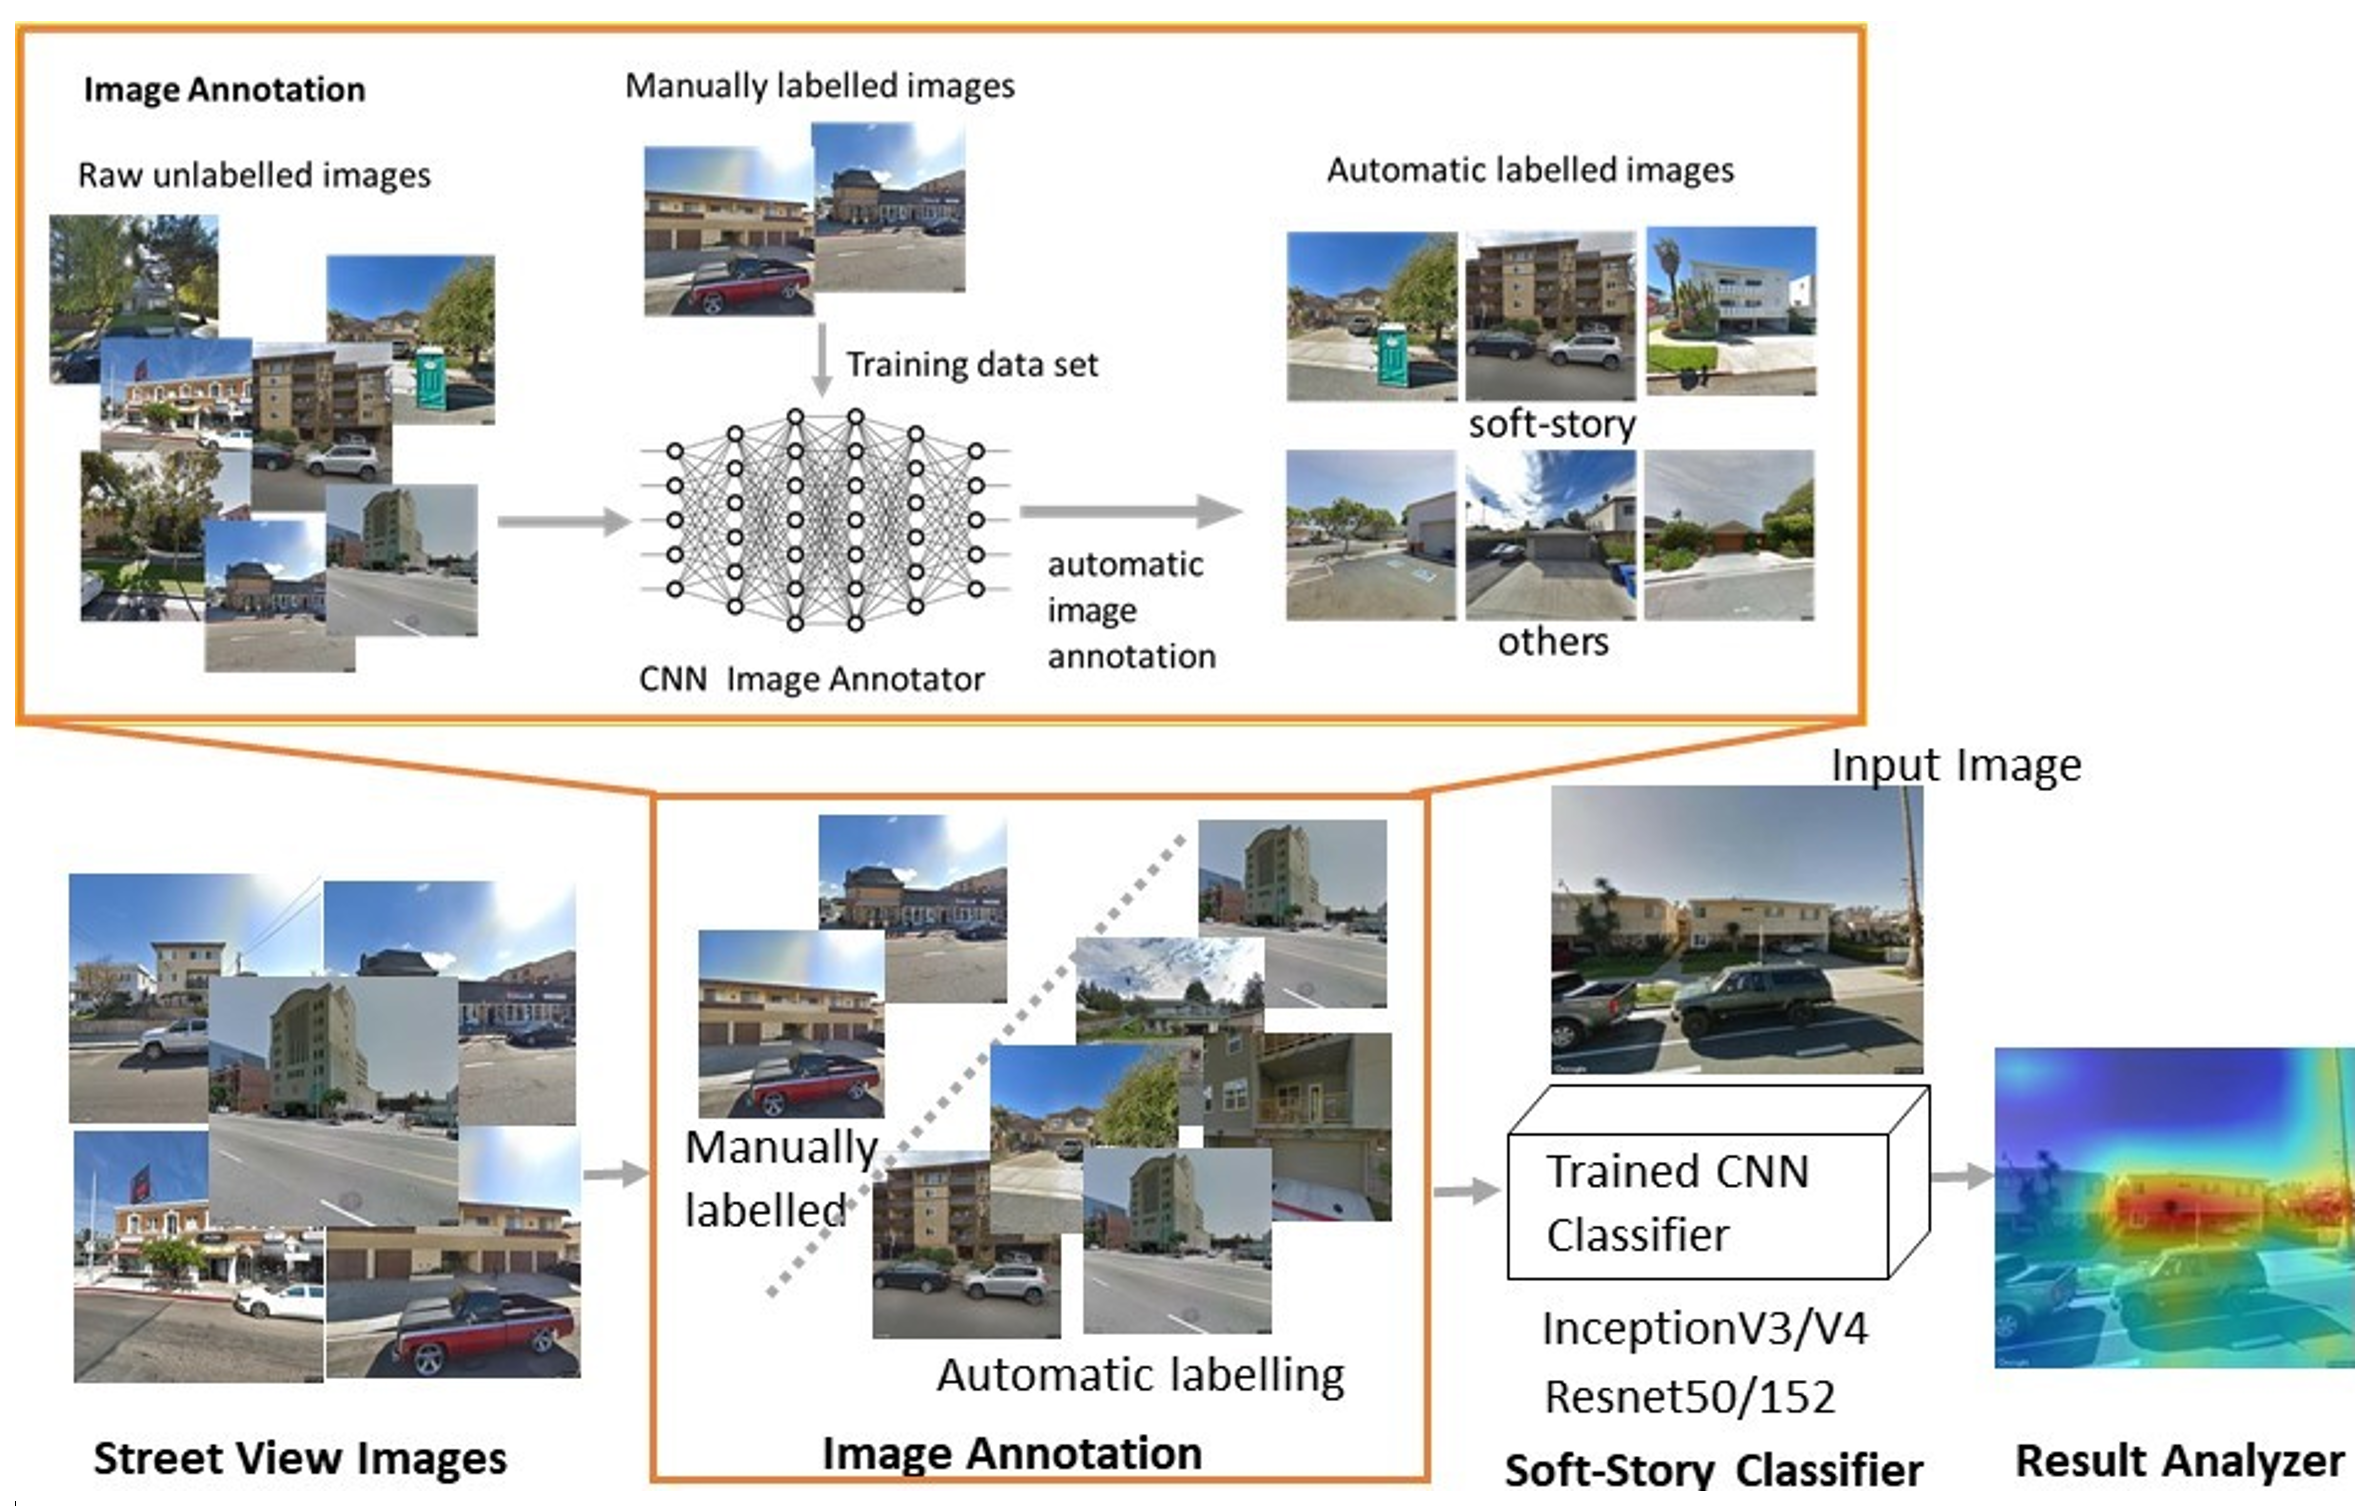
\includegraphics[width=1.0\textwidth, angle = 0]{Figures/soft_story_identification.png}
    \caption{A Workflow Framework for Soft-Story Identification}
    \label{fig:soft_story_identification}
\end{figure}

\subsection{Regional-Scale Natural Hazard Risk Management }

Many environmental and geographical models, such as those used to understand regional hazards and those used in climate studies, often rely on spatially distributed data as input that are known to be scarce and imperfect. Generally, there is a lack of knowledge about the distribution pattern of the variables over the spatial area in the region. In other words, spatial uncertainties exist because of noise, incompleteness, and the uncertainties in the data. For regional risk analyses, spatial uncertainties in the input data, such as the hazard intensities or asset attributes, can propagate into model predictions across the whole region. To quantify such uncertainties, SimCenter has developed a Spatial Uncertainty Research Framework, SURF (Wang, 2019). The framework has been implemented as a Python package for performing spatial uncertainty analysis using random fields and neural networks. Given a spatially scattered dataset, SURF learns the variation patterns in the dataset and infers missing attributes and values where there are no observations. 

For regional hazard evaluation, an important first step is to collect the relevant information of existing buildings and to establish an inventory of buildings in the region. Attributes of a building, such as the number of stories, the year of construction, structure type, occupancy type, and others, are important parameters to assess the effects of natural hazards on the building structure. Many of these textual building attributes are available as public information, for example, from the tax assessor records. However, the building record is often incomplete with missing data. Furthermore, key attributes (e.g., roof types) needed for specific hazard assessment studies are often not recorded. With the availability of street view and satellite images and other open data sources, recent advances in computing technologies, including computer vision, geospatial analytics, and machine learning, can help bridge the information gaps for regional hazard modeling and risk analysis. To this end, SimCenter has initiated a building information modeling project, BRAILS (Wang and Yu et al., 2019). BRAILS (Building Recognition using AI at Large Scale) is a tool that employs ML/DL methods to help create building inventories at the city or regional scale.

As illustrated earlier, deep learning methods can be applied to screen seismically vulnerable buildings by capturing buildings' visual cues with geometric irregularities\citep{yu2020}. Similarly, many building attributes, such as structural and material types, can be "learned" and identified using the observable cues from building images via machine learning. For instance, CNN is shown to be effective in classifying roof shapes (flat, gabled, or hipped) using satellite images (Wang and Yu et al., 2020). In addition to extracting attribute information using individual building images, machine learning can also infer missing building information using geospatial patterns in the region of interest. To develop a geospatial learning module, the aforementioned Python package (SURF) is encoded as a part of the BRAILS framework, which has been designed for regional hazard analysis (Wang, 2019). 

Figure \ref{fig:AI_workflow_for_regional_analysis} shows the BRAILS workflow for the building inventory development process for regional hazard risk analysis (Wang and Yu et al., 2020). The workflow infers building information from multiple sources (e.g., tax assessment, street view images, satellite images, etc.) to form a large database of building inventory. For example, in one of the testbeds, the coastal cities in New Jersey are selected to assess the effects of high wind and hurricanes on the region's buildings. The data sources included the tax assessor records, Microsoft's Building Footprints dataset, and street view and satellite images obtained using Google Maps API. The textual data from tax assessor records and the information inferred from images using convolutional neural networks are aggregated or "fused" to establish the building information needed by the damage models and fragility functions defined in FEMA's HAZUS MH2.1 (FEMA, 2018). The source code, the data, the pre-trained CNN models, and the building inventory database are available at SimCenter's repository (Wang and Yu et al., 2019). The key significance of this effort is to create an AI/ML-based workflow from data acquisition, building information model development, hazard modeling to spatial hazard risk analysis. 

\begin{figure}[htb]
    \centering
    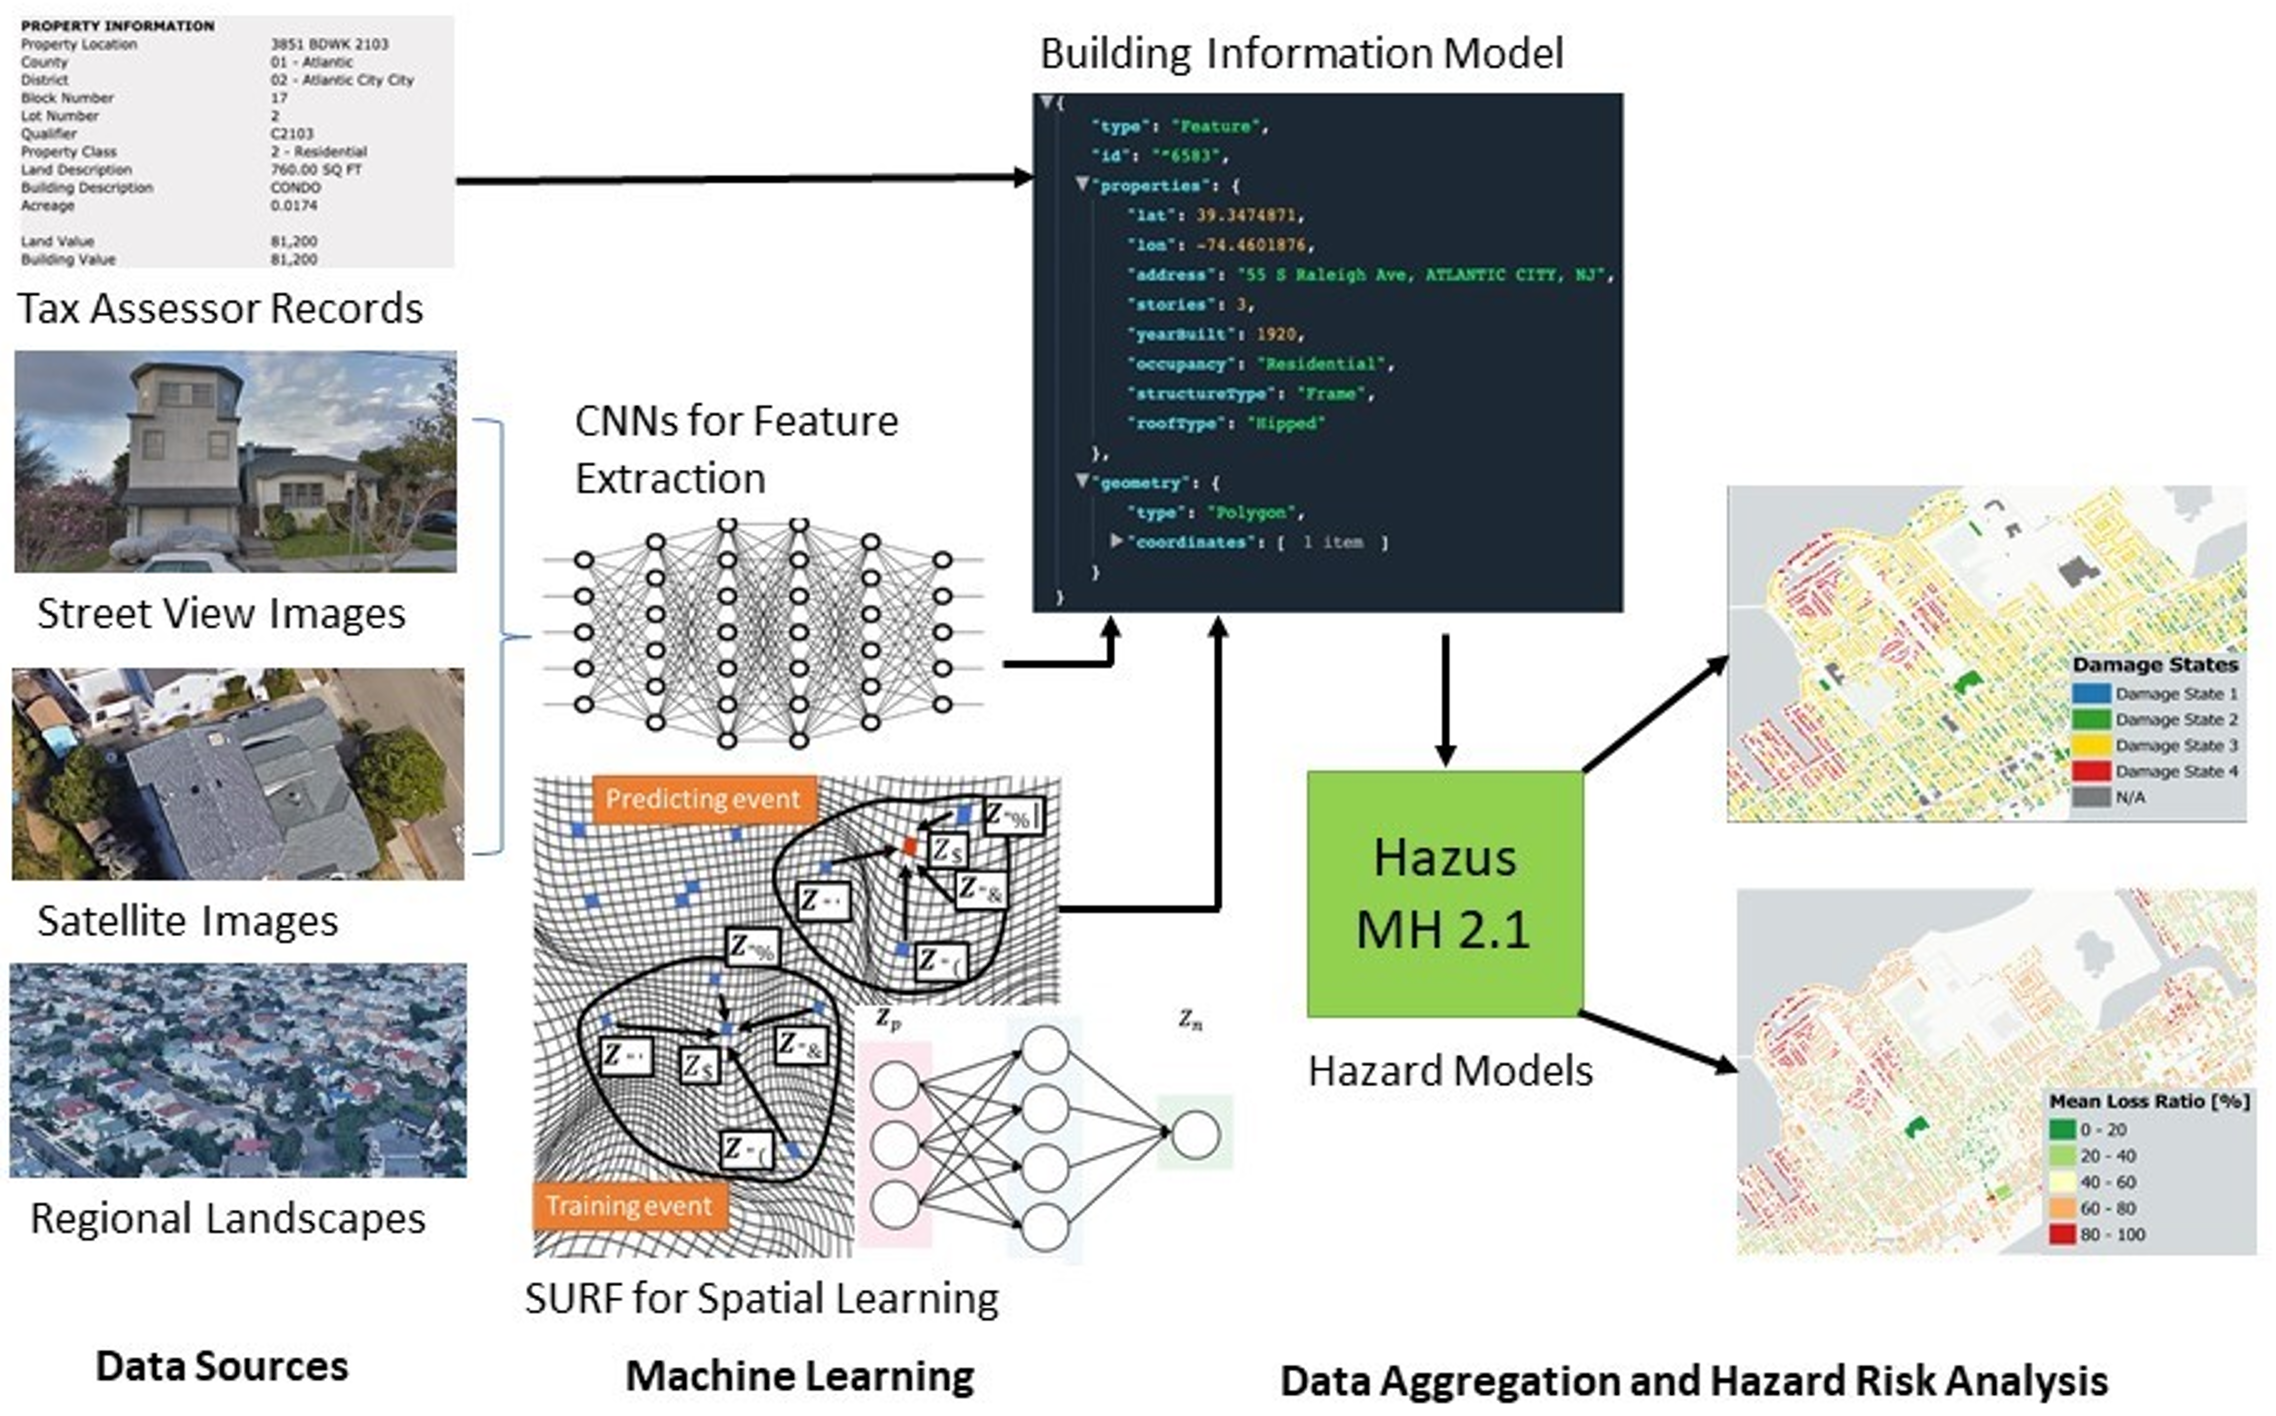
\includegraphics[width=1.0\textwidth, angle = 0]{Figures/AI_workflow_for_regional_analysis.png}
    \caption{A Workflow Framework for Regional Hazard Modeling and Analysis}
    \label{fig:AI_workflow_for_regional_analysis}
\end{figure}

\section{Research Challenges and Opportunities}
\label{sec:ai_gaps}

Applications of AI/ML to NHE are numerous, in that almost all facets of NHE, across each task of NHE and for each type of natural hazard, can potentially be benefited from AI/ML. For instance, instead of traditional physics-based representations, material constitutive models can be represented using ML models (such as SVR, ANN, GPR, or DL), which can self-adapt and "learn" with new data. At the large scale, ML can be (and have been) used to understand human behaviors (such as evacuation), social structure (such as the population residing in an area), and environmental and hazard conditions (such as wind intensity and seismicity) that could have implications on regional NHE decision-making processes. While the field of AI/ML in NHE is too broad to enumerate, this report brings forth three general issues that could enhance the adoption and facilitate the development of AI/ML in NHE. First, an AI/ML model should be able to provide explanations of the outcomes, that will help build the users’ trust and confidence in the model. Second, while an ML model, once trained or built adaptively with new information, can be incorporated as a "surrogate" and used efficiently in a larger simulation or optimization setting, the limitations and the uncertainties that can potentially propagate to the system need to be addressed. Lastly, as significant amounts of relevant and labeled data are necessary to build even the baseline AI/ML models in support of NHE, the data issues from acquisition to management, require new approaches and a collaborative community effort to enable progress and advancements in this field. 

\subsection{Explainable and Physics-Informed AI/ML}

Early AI works such as knowledge-based expert systems have inherent inference mechanisms that can be used to explain how a system leads to a conclusion based on the rules and knowledge executed. For instance, incorporated with handcrafted rules and first principles, SACON\citep{bennett1978}—an expert consultant system for structural analysis that was built upon the EMYCIN framework (van Melle, 1984)—could not only recommend an appropriate analysis class for solving a given engineering problem but also provide associated explanations for the specific recommendation. While deep learning methods (such as multi-layered neural networks) have been shown superior and capable of solving many complex and difficult problems where it is infeasible to write down the explicit rules, they are often criticized as black box models that lack transparency. It is not always clear how a machine learning model reaches a decision. Developing machine learning models that can provide contextual explanation, interpretation, and induction of the model is challenging; and thus, it is exceedingly important to validate the models and justify their use with hindcasting-type studies (darpa2016explainable; Samek et al., 2019; Rudin and Radin, 2019). AI/ML models that are unable to adequately answer questions on how a problem is solved and why a conclusion is made may suffer trust and confidence issues in practice. The users may hesitate to deploy these models and utilize their results. Naturally, ML-based models that lack the ability to explain their output and interpret their own performance will likely encounter skepticism and hindered adoption in natural hazard engineering. 

Many active research efforts are now underway that aim to enhance our understanding of why AI/ML techniques work well in practice, what classes of problems AI/ML are capable of solving, and which AI/ML algorithms are particularly effective on certain types of problems. The advancements in attention-based methodologies, which mimic human cognition and intuition, have enabled tools to recognize the important features of a trained model and highlight the results generated by the model \citep{Xu2015show,zhou2016learning,kafle2017visual,nakka2018deep}. The highlighted results, for example, could help a user to gain insights about the ML-trained model, trace the features involved in the correct (or incorrect) identification of the results, and assess the relevance of the information that propagates through the model. Graph-based methodologies that are able to incorporate domain concepts and features into machine learning models have also attracted much attention (koller2009probabilistic; Nickel et al., 2016,baru2017open,hamilton2017representation,u2020comprehensive}. For instance, graph neural networks are now widely used in bridging machine learning methodologies with modeling of engineering problems (Seo and Liu, 2019; Park and Park, 2019). The feature information embedded in graph-based models can help construct interpretable models, enhance the reasoning process, and ensure the quality of the generated results. 

The ability to interpret the results and to explain the trained model using domain terminologies is important to encourage the adoption of ML methods. Traditionally, engineering models are developed using fundamental principles of physics or other fields of science and statistically validated with experimental data and empirical evidence. For obvious practical reasons, engineering models are often simplified to lessen the complexity of physical phenomena and to allow the selection of model parameters that are measurable. On the other hand, ML models constructed using data can often perform well even for complex problems; but their inferences, as discussed above, are hard to explain, and the models are difficult to generalize. One common approach is to evaluate a machine learning model based on qualitative interpretation and quantitative correlation between the behavior of the trained ML model and the physical system. For example, Kratzert et al. (2019) show the interpretation of LSTM (long short-term memory) for a rainfall-runoff model by examining the outputs of the LSTM network based on the domain knowledge about the annual variation of the hydrological pattern and the correlation between the memory cells of the LSTM network with the physical state of the hydrological system. Linking the relationships between the ML model and the physical problem is important to realize the significance of the outputs and gain confidence over the results. 

Recently, much research efforts have been dedicated to taking advantage of first principle domain knowledge and machine learning methodologies by combining the data and the domain features when training a machine learning model \citep{willard2020integrating}. The research typically focuses on two basic themes: (1) To what extent should first principle knowledge be embedded in an ML model, and (2) how the features of the physical system and the first principles be incorporated in the training process. For instance, using examples in turbulence modeling and crystal plasticity, Ling et al. (2016) discussed how symmetric and invariance properties inherent in physical systems could be incorporated and learned by ML algorithms such as random forests and deep neural networks. Another approach is to train the ML-models in accordance with physical laws, which are described, for example, by differential equations \citep{raissi2019physicsinformed}. One advantage of a physics-based ML model is that it may be possible to assess the model parameters' uncertainties using the data collected from sensor measurements on the physical systems \citep{zhang2019quantifying}. One other approach is to augment an ML method with physics-based features such that these features penalize inconsistencies with the laws of physics (e.g., conservation of momentum), for example, using an appropriately devised loss function during the training process \citep{jia2020physicsguided}. This physics-guided approach has been demonstrated for simulating the temperature profile of a lake using sparse observation data while achieving high-prediction accuracy. Methods that incorporate first principle knowledge into the training of ML models could provide the basis needed for verification and validation and ensure that the models are consistent with the physical systems. 

Explainability and interpretability of machine learning models are important for their adoption in natural hazards engineering. Further studies are needed to set the foundations in this field. In a broader context, research in explainable ML models advocates fruitful synergy and provides ample opportunities for collaborations between AI/ML researchers and domain experts in NHE.

\subsection{Surrogate Modeling}

Particularly in the last decade, the number of surrogate modeling studies involving data-driven methods has seen a steady increase in NHE. Despite differences in the ML methods utilized, these efforts share a common goal. They aim at creating computationally efficient alternatives to procedures that are otherwise too resource-intensive for the considered application (which, typically, requires large scale simulations as in regional-level loss assessment predictions). These studies range from surrogate model development efforts for peak or time-dependent storm surge prediction based on high fidelity hydrodynamic model outputs \citep{jia2016surrogate} to deck unseating fragility of bridges subjected to hurricane-induced wave loading developed using the results of nonlinear fluid-structure interaction simulations \citep{ataei2015fragility}. However, the concentration of these studies across the sub-domains of NHE is not uniform. Most surrogate modeling studies focus on flood forecasting. In some areas, such as earthquake engineering, the research is at its initial strides. Whereas, some potential areas of geotechnical engineering, e.g., surrogate models for rock engineering, are practically uncharted.

Virtually all of the existing data-driven surrogate modeling studies in NHE rely on simulated data. Hence, in the process of creating computationally-efficient representations of processes, the use of surrogate models may increase epistemic (model) uncertainties, depending on the ability of the training data to cover the entire domain of the modeled process and the capability of the ML method used to capture the underlying mechanisms from this data without overfitting. Model uncertainties are significant for many NHE problems \citep{gokkaya2016quantifying}; yet, perhaps, due to the long-standing research gap in this area, limited attention is paid to the uncertainty associated with data-driven surrogate models and the effects of the uncertainties to the overall system.

In recent years, key advancements were made in uncertainty quantification for neural network-based learning methods. As a direct outcome of these developments, various accepted practices continue to come into existence. The confidence interval determination methods summarized by Kabir et al. (2018) provides a snapshot of the procedures for determining uncertainties associated with neural network models. Many successful implementations of the ideas presented in this work exist in finance, medicine, and control systems applications. Bayesian Neural Networks \citep{blundell2015weight} are another alternative that enables the assessment of uncertainties in neural network models. McDermott and Wikle (2019) demonstrated that the practical implementation of Bayesian Neural Networks to different network architectures, such as recurrent neural networks, is possible. 

So far, translation of the recent progress in uncertainty quantification for neural network-based methods and machine learning models in general, to surrogate modeling of NHE processes remains a largely unexplored territory. Given the computational foundations of such studies are in the act of getting established, ample opportunities stand open for further research.

\subsection{Data Generation and Management}

Data plays an indispensable role in NHE and machine learning. There are at least three categories of information commonly employed in NHE – assets of the built infrastructures, models of the natural hazards, and geospatial information about the built, natural, and socioeconomic environments. For instance, in addition to the physical architectural (such as footprints, exterior walls, roof shapes, openings) and structural (such as materials, framing systems) information, other attributes of buildings such as year built and property values may contribute to the evaluation of structural integrity and affect the decision making on retrofitting and repair strategies. Environmental information such as wind speed and direction, weather conditions, seismicity, etc. may be required for the hazard simulation models. Geospatial data/metadata about the terrain, vegetation, and landscapes, proximity to water bodies, nearby highways and lifeline networks, are essential to regional hazard evaluation. Socioeconomic data—such as residential, commercial, and industrial zonings, tax assessments, and real estate values—could play a part in regional impact and risk analyses, and emergency planning. Different data sets and different types of data are needed for different hazard models and for the different objectives and purposes of NHE evaluation. A typical data collection process involves identifying available data from public and private sources, getting access to the data, and integrating the data in a meaningful way that is suitable for the tasks at hand. Gathering high quality and well organized useful data is often the most time consuming and challenging task in NHE research. Indeed, the data issue has often been considered one of the main impediments in NHE studies. 

Natural hazard engineering (NHE), particularly at a regional scale, requires a wide variety and large volume of data. There exist many ongoing data initiatives, such as those towards developing digital twins for smart cities (NIC, 2017; lehner2020digital; Schrotter and Hürzeler, 2020; day2019bentley). While such efforts, which often involve computer vision, sensing, and machine learning technologies, could potentially help create useful digital data and providing geometric descriptions of the built environment in a city or a region in the future, many significant research challenges remain in gathering and creating the data needed for NHE studies as well as in managing and facilitating access to the data. Presently, NHE researchers rely heavily on publicly accessible data sets, such as building inspection files and tax assessor records. To date, many of such data are collected and gathered manually and entered manually into databases (with tools such as Excel, Access, etc.), often with subjective judgments and interpretations. Despite the best intentions and efforts from all parties involved, erroneous entries and missing information are common. Information specific to NHE, such as material types, roof types and geometry, building configuration, are often not recorded. ML can be a valuable tool to generate and fill in some of the data needed to support NHE applications. 

For certain problems and data types, an ML model can be developed and applied to enhance data quality, augment existing data sets, and create new data sets useful for NHE applications. For example, ML methods, combined with engineering simulations, can potentially be applied to cross-check field measurement data. Methods, such as principal component analysis (PCA), support vector regression (SVR), recurrent neural network (RNN), have been shown capable of identifying erroneous measurements and reconstructing vibration signals (kerschen2005sensor,jeong2019sensor}. Kriging has been combined with statistical-based methods to estimate wind speeds and extrapolate information at locations that are not physically measured (Xu et al. 2014). Historical (analog) seismic records can be converted to useful digital seismic signals using deep learning (Wang and Ellsworth et al., 2019). Machine learning has the potential to ensure data quality and provide estimates (or predictions) on some of the missing attribute data that are critical to NHE simulations. While developing ML models often requires a large amount of labeled data, active and assistive learning strategies can help alleviate some of the time consuming and laborious annotation efforts and build useful ML models (joshi2009multiclass,wong2019assistive,yu2020largescale}. 

One of the main challenges in regional hazard analysis is to establish an inventory of assets and their properties over a geospatial area of interest. With advances in computational geometry, computer vision, and machine learning, street view, satellite, and aerial images are tremendous data sources that can be used to acquire 2D and 3D building geometry metadata and to extract other valuable information about the buildings and their surrounding environment. For instance, semantic segmentation and polygonalization of aerial images have produced over 125 million building footprint geometries in the US (https://github.com/microsoft/USBuildingFootprints). Similar techniques can be used to help identify other building attributes, such as garages, windows, number of floors, structural materials, and other meaningful metadata. Depending on the levels of details (LoD) required for a specific NHE application, different computational algorithms and AI/ML methodologies have been proposed to construct 3D building models. For instance, 3D block models (consisting of building envelope and roof geometry) can be extruded from footprint data and machine learning edge extraction techniques (maninis2017convolutional,yu2017casenet}. Such 3D block models could be useful for low fidelity NHE simulations or prescriptive code-based analyses. Many active ongoing research efforts, utilizing a combination of computational geometry algorithms, machine learning methods, rule-based inferences that incorporate design and planning principles, are underway that aim to construct detailed building information models (martinovic20153d,chen2018automatic}. The generated models that have detailed descriptions of the buildings—including materials, windows and openings, roof shapes, and chimneys—can be used for conducting high fidelity computational simulations such as nonlinear structural analyses and CFD studies. In short, AI and machine learning can find ample applications to help build data inventory necessary for NHE modeling and analyses, as well as for training and testing ML models. 

Numerous current efforts have focused on collecting and generating data for individual simulation applications and for machine learning model development. The challenges in achieving tangible advances in NHE go well beyond the abilities of individual researchers or even organizations and require well-coordinated community efforts. The significant impacts of having made large datasets—such as ImageNet \citep{deng2009imagenet} and COCO \citep{lin2014microsoft}—publicly available on advancing the fields of computer vision and machine learning cannot be understated. Within the NHE domain, open-source tools, such as OpenSees \citep{mckenna2011opensees} and OpenFoam\citep{chen2014}, have greatly facilitated research and developments in earthquake and wind engineering. The current community-driven initiative in making NHE data accessible on the DesignSafe CyberInfrastructure platform is an effort that will help expedite progress in this field\citep{rathje2017}. To promote, encourage, and facilitate the adoption of AI and ML research in NHE, a community-based platform, analogous to the "model zoo" established in the machine learning community (see https://github.com/collections/ai-model-zoos), that allows publishing and sharing of ML models and data sets that are specific to the NHE domain will be useful. 

Even when researchers and organizations are willing to share and make their data and models available publicly, the data objects (i.e., the data and the models) need to be ``Findable, Accessible, Interoperable and Reusable (FAIR)'' \citep{wilkenson2016fair}. Metadata constructed using standardized representation, authorization, and authentication protocols can play a key role in improving on the FAIR quality of data. ML and NHE applications have to "understand the data" in order to use the data for training and engineering simulations. Metadata and domain ontologies will enable data shareability, interoperability and usability, and advances in ML and NHE. For instance, BioPortal, enabled with an ontology authoring and accessing tool Protégé, has provided researchers and interested users access to a library of biomedical ontologies and terminologies, that, in turn, has facilitated a broad spectrum of medical research activities \citep{whetzel2011bioportal}. Semantic web technologies—such as RDF, OWL, SPARQL, and other tools (see https://www.w3.org/standards/semanticweb/ for details)—can help define, publish, link, and query data objects. Recently, knowledge graphs, a representation for capturing data objects and their relations describing a domain or a field of study, have been proposed to manage and to facilitate retrieval of unstructured data objects, such as video, images, audio, and text, that do not fit neatly into the tabular structure of relational databases (Paulheim, 2016,bonatti2018knowledge,reinanda2020knowledge}. The traversable graph representation allows search and access to different data objects and enables the fusion of information from different sources. Knowledge graphs have also been shown great promise to integrate with machine learning \citep{lin2018multihop}. Developing and managing data, models, and knowledge bases is an expensive endeavor. To alleviate some of the burdens on individual communities or organizations, Open Knowledge Network is one recent movement that attempts to build an open national-scale domain-agnostic infrastructure accessible to a broad community \citep{baru2017open}. The open infrastructure has the potential to drive innovation across science and engineering and allows data sharing within and outside a specific domain such as NHE.

In summary, at the core of machine learning methods and many aspects of NHE is data. To enable advances in AI/ML and NHE, the availability of large volumes of high quality and relevant data is essential. Using existing data and knowledge about those data, the ML methods can, at times, build models that can help generate new (possibly labeled) data needed to train ML models and to support NHE applications. A common open platform that can attract a broad base community involvement will be useful to promote collaborations and encourage the sharing of data and models. The adoption of semantic technologies will potentially further enhance data accessibility and model interoperability and further facilitate the research and development as well as deployment of AI/ML in NHE. 

\section{Summary and Discussion}
\label{sec:ai_summary}

AI/ML is poised to bring significant transformational changes to scientific research and engineering practice. Although the potential applications of AI/ML in NHE is enormous, the field is still in its infancy. This report aims to provide a glimpse of the possibilities of applying AI/ML technologies in NHE, to encourage collaborations between NHE and AI/ML researchers, and to engender further research and developments in this promising field. However, many open questions and barriers remain that may deter the pace of progress and the adoption of the technologies in practice. 

First, just like any new technological advancements, there should not be any unrealistic expectations by the NHE researchers and practitioners about the applicability of AI/ML technologies. While research and exploration of AI/ML and its applications in NHE are encouraged, their misuse and flawed developments can quickly draw disproportionate criticisms within the NHE community and hinder advancements in the field. While statistics-based measures—such as root-mean-square-error, precision, recall, F1 scores, mean IoU, and other metrics—are commonly used to assess ML model accuracy, proper verification and validation of their results based on engineering knowledge and professional judgment remain valuable. It should be cautioned that an accurate deep learning model does not necessarily imply a good model in practice \citep{mignan2019forecasting}. Furthermore, a model trained using a data set (say, obtained in a residential neighborhood) may not necessarily generalizable to data (say, from a commercial area) that differs from the training set, even within the same domain of interest. In other words, AI/ML does not diminish the importance of the fundamental knowledge and professional know-how in NHE. Additional research is needed to develop a broad spectrum of evaluation techniques that include standards, benchmarks, and testbeds. Most importantly, community engagement is essential to guide and evaluate progress. 

Advancements in this field require a strong and well-trained community of researchers from both AI/ML and NHE. The demands for developing such a community entail educating a new generation of NHE researchers and practitioners who become well-versed in AI/ML. Researchers in NHE should acquire a knowledge of AI and machine learning methods and understand the applicability of the technologies and their limitations. Synergistic and genuine collaborations between NHE and AI/ML researchers are necessary in order to foster new and innovative solutions as advances in AI/ML will continue to grow rapidly in years to come. 

\section{Relevant AI/ML Software}
\label{sec:ai_tools}

With the growing interests and importance of AI/ML in academic research and commercial developments, universities and companies have built a number of frameworks and tools that are now used by researchers and practitioners to build and execute AI/ML models. Both Matlab and Mathematica, the computational tools commonly used in education settings, have ML and DL toolboxes. Cloud service vendors, such as Amazon AWS, Google Cloud, Microsoft Azure, IBM, Oracle, and others, all have machine learning platforms that support end-to-end model training and executing (scoring) functions. 

In addition to commercial platforms, examples of open machine learning frameworks and tools publicly available include:
\newline

\noindent\textbf{Scikit-learn} (also known as sklearn) \\https://scikit-learn.org, https://github.com/scikit-learn/scikit-learn\\Originally developed as a Google Summer of Code project, Scikit-learn is a free software machine learning library that features a collection of statistical-based machine learning algorithms for classification, regression, and clustering, such as support vector machines, random forests, k-means, decision trees, and numerous others. The library is designed to interoperate with Python numerical and scientific libraries, NumPy and SciPy. 
\newline

\noindent\textbf{CAFFE} (Convolutional Architecture for Fast Feature Embedding) \\https://caffe.berkeleyvision.org/, https://github.com/BVLC/caffe \\Originally developed at UC Berkeley, CAFFE is an open-source deep learning framework, written in C++, with a Python interface, featuring CNN, RCNN, LSTM, and other deep neural networks and specializing in computer vision, and image classification and segmentation. It is no longer actively developed though CAFFE2 was merged into PyTorch in 2018.
\newline

\noindent\textbf{TensorFlow} \\https://www.tensorflow.org/, https://github.com/tensorflow/tensorflow \\Originally developed by the Google Brain team, TensorFlow is a free and open-source software library for high-performance numerical computation and dataflow and differentiable programming. Its flexible architecture allows easy deployment of computation across various platforms (CPUs, GPUs, TPUs). TensorFlow is commonly used to develop machine learning applications, such as deep neural networks.
\newline

\noindent\textbf{PyTorch} \\https://pytorch.org/, https://github.com/pytorch/pytorch, \\Primarily developed by Facebook's AI Research Lab, PyTorch is an open-source machine learning library (based on the Lua-Torch library) with Python and C++ interface, featuring accelerated tensor computing on GPU and deep neural networks built on automatic differentiation system. PyTorch also supports CAFFE2, a version of CAFFE. PyTorch has been used for applications such as computer vision and natural language processing. 
\newline

\noindent\textbf{Microsoft Cognitive Toolkit} (CNTK) \\https://docs.microsoft.com/en-us/cognitive-toolkit/, https://github.com/microsoft/CNTK \\Developed by Microsoft Research, Microsoft Cognitive Toolkit (CNTK) is an open-source toolkit for distributed deep learning with parallelization across multiple GPUs and servers. CNTK describes neural networks as a series of computational steps via a directed graph and allows users to easily realize and combine popular model types such as feed-forward DNNs, convolutional neural networks (CNNs), and recurrent neural networks (RNNs/LSTMs).
\newline

\noindent\textbf{Theano} \\http://deeplearning.net/software/theano/, https://github.com/Theano/Theano \\Developed at the University of Montreal, Theano is a Python library and optimizing compiler for manipulating and evaluating mathematical expressions, efficiently on either CPU or GPU architectures, and supports machine learning application developments. 
\newline

\noindent\textbf{Keras} \\https://keras.io/, https://github.com/keras-team/keras \\Developed as part of the research project ONEIROS (Open-ended Neuro-Electronic Intelligent Robot Operating System) at Google, Keras is an open-source neural network library written in Python. It offers a higher-level, and an intuitive set of abstractions that make it easy to develop deep learning models regardless of the computational backend used. It is capable of running on top of TensorFlow, Microsoft Cognitive Toolkit, R, Theano, and other platforms. Keras is supported in Tensorflow's core library. 
\newline

Note that all of these tools are publicly available. Additionally, a large number of machine learning and deep learning models developed using the open-source frameworks can be found at https://github.com/collections/ai-model-zoos.

\section{References}

%TODO: These are the references that need to be added to the references.bib file
%
%Abbot, J., and Marohasy, J. (2014). "Input Selection and Optimisation for Monthly Rainfall Forecasting in Queensland, Australia, Using Artificial Neural Networks," Atmospheric Research 138:166–178.
%
%Alimoradi, A., and Beck, J.L. (2015). "Machine-Learning Methods for Earthquake Ground Motion Analysis and Simulation," Journal of Engineering Mechanics, 141 (4): 04014147.
%
%Aquino, W., and Brigham, J.C. (2006). "Self Learning Finite Elements for Inverse Estimation of Thermal Constitutive Models," International Journal of Heat and Mass Transfer, 49:2466-2478.
%
%Ataei, N., and Padgett, J.E. (2015). "Fragility Surrogate Models for Coastal Bridges in Hurricane Prone Zones," Engineering Structures, 103, 203–213.
%
%ATC (2015). A Handbook for Rapid Visual Screening of Buildings for Potential Seismic Hazards, FEMA 154, 3rd Edition, Federal Emergency Management Agency, Washington, D.C..
%
%Bai, Y., Adriano, B., Mas, E., and Koshimura, S. (2017). "Machine Learning Based Building Damage Mapping from the ALOS-2/PALSAR-2 SAR Imagery: Case Study of 2016 Kumamoto Earthquake," Journal of Disaster Research, 12 (sp): 646–655.
%
%Baru, C. (2017). "Open Knowledge Network: Recap & Some Related Work at NSF," presented at the Open Knowledge Network – Enabling the Community to Build the Network, National Institute of Health.  (Available at https://www.nitrd.gov/nitrdgroups/images/c/ca/OKN_ChaitanBaru.pdf)
%
%Bennett, J., Creary, L., Englemore, R., and Melosh, R. (1978). SACON: A Knowledge-Based Consultant for Structural Analysis, Technical Report STAN-CS-78-699, Stanford University.
%
%Bishop, C.M. (1995). Neural Networks for Pattern Recognition, Oxford University Press.
%
%Blundell, C., Cornebise, J., Kavukcuoglu, K., and Wierstra, D. (2015). "Weight Uncertainty in Neural Network," Proceedings of the 32nd International Conference on Machine Learning, Proceedings of Machine Learning Research, PMLR, Lille, France, 1613–1622.
%
%Bonatti, P.A., Decker, S., Polleres, A., and Presutti, V. (2018). "Knowledge Graphs: New Directions for Knowledge Representation on the Semantic Web," Dagstuhl Reports, 8(9): 29-111.
%
%Cha, Y.J., Choi, W., and Buyukozturk, O (2017). "Deep Learning-Based Crack Damage Detection Using Convolutional Neural Networks," Computer Aided Civil and Infrastructure Engineering, 32(5):361-378.
%
%Chen, G., Xiong, Q., Morris, P.J., Paterson, E.G, Sergeev, A., and Wang, Y.-C. (2014). "OpenFOAM for Computational Fluid Dynamics,” Notices of the American Mathematical Society. 61 (4): 354–363. doi:10.1090/noti1095
%
%Chen, K., Lu, W., Xue, F., Tang, P., and Li, L.H. (2018), "Automatic Building Information Model Reconstruction in High-Density Urban Areas: Augmenting Multi-Source Data with Architectural Knowledge," Automation in Construction 93:22–34.
%
%Cohn, L.F., and Harris, R.A. (1992). Knowledge-Based Expert Systems in Transportation, Synthesis of Highway Practice 183, Transportation Research Board.
%
%Cooner, A.J., Shao, Y., and Campbell, J.B. (2016). "Detection of Urban Damage Using Remote Sensing and Machine Learning Algorithms: Revisiting the 2010 Haiti Earthquake," Remote Sensing, 8 (10): 868.
%
%Darabi, H., Choubin, B., Rahmati, O., Haghighi, A.T., Pradhan, B., and Kløve, B. (2019). "Urban Flood Risk Mapping Using the GARP and QUEST Models: A Comparative Study of Machine Learning Techniques," Journal of Hydrology, 569: 142–154.
%
%DARPA (2016), Explainable Artificial Intelligence (XAI), Broad Agency Announcement, DARPA-BAA-16-53.
%
%Day, M. (2019), "Bentley on Digital Twins," AEC Magazine. (Available at https://www.aecmag.com/component/content/article/59-features/1910-bentley-on-digital-twins
%
%Deng, J., Dong, W., Socher, R., Li, L.-J., Li, K., and  Li, F.-F. (2009). "ImageNet: A Large-Scale Hierarchical Image Database," IEEE Computer Vision and Pattern Recognition (CVPR). 
%
%Dou, J., Oguchi, T., Hayakawa, Y.S., Uchiyama, S., Saito, H., and Paudel, U. (2014). "GIS-Based Landslide Susceptibility Mapping Using a Certainty Factor Model and Its Validation in the Chuetsu Area, Central Japan," In Landslide Science for a Safer Geoenvironment, 419–424. Springer.
%
%Dym, C.L., and Levitt, R.E. (1991).  Knowledge-Based Systems in Engineering, McGraw Hill, NY.
%
%Eriksson, D.M. (2018).  Scalable Kernel Methods and Their Use in Black-Box Optimization, PhD Thesis, Cornell University.
%
%FEMA (2018). HAZUS-MH2.1 Hurricane Model Technical Manual, Federal Emergency Management Agency, Washington, D.C..
%
%Ferguson, M., Ak, R., Lee, Y.-T.T., and Law, K.H. (2018). "Detection and Segmentation of Manufacturing Defects with Convolutional Neural Networks and Transfer Learning,” Smart and Sustainable Manufacturing Systems. 2(1):137-164. 
%
%Gao, Y., and  Mosalam, K. M. (2018a). “Deep Transfer Learning for Image-Based Structural Damage Recognition,” Computer-Aided Civil and Infrastructure Engineering, 33(9), 748– 768.
%
%Gao, Y., and  Mosalam, K.M. (2018b). Structural ImageNet and PEER Hub ImageNet Challenge 2018. 10.13140/RG.2.2.33674.77766.  (see https://apps.peer.berkeley.edu/phi-net/)
%
%Garrett, Jr., J.H., and Smith, I.F.C. (1996). "AI Applications in Structural/Construction Engineering," IEEE Expert, 11(3):20-22. 
%
%Gebrehiwot, A., Hashemi-Beni, L., Thompson, G., Kordjamshidi, P., and Langan, T.E. (2019). "Deep Convolutional Neural Network for Flood Extent Mapping Using Unmanned Aerial Vehicles Data," Sensors, 19 (7): 1486.
%
%Ghaboussi, J., Garrett, Jr J., and Wu X. (1991). "Knowledge-Based Modeling of Material Behavior with Neural Networks," Journal of Engineering Mechanics, 117(1):132–153.
%
%Ghaboussi, J., Pecknold, D.A., Zhang, M., and Haj-Ali, R.M. (1998). "Autoprogressive Training of Neural Network Constitutive Models," International Journal for Numerical Methods in Engineering, 42:105-126.
%
%Ghorbanzadeh, O., Blaschke, T., Gholamnia, K., Meena, S.R., Tiede, D., and Aryal, J. (2019). "Evaluation of Different Machine Learning Methods and Deep-Learning Convolutional Neural Networks for Landslide Detection," Remote Sensing, 11 (2): 196.
%
%Gidaris, I., Taflanidis, A.A., and Mavroeidis, G.P. (2015). "Kriging Metamodeling in Seismic Risk Assessment Based on Stochastic Ground Motion Models," Earthquake Engineering & Structural Dynamics, 44 (14): 2377–2399.
%
%Gizaw, M.S., and Gan, T.Y. (2016). "Regional Flood Frequency Analysis Using Support Vector Regression under Historical and Future Climate," Journal of Hydrology, 538: 387–398.
%
%Goetz, J.N., Brenning, A., Petschko, H., and Leopold, P. (2015). "Evaluating Machine Learning and Statistical Prediction Techniques for Landslide Susceptibility Modeling," Computers & Geosciences, 81: 1–11.
%
%Gokkaya, B.U., Baker, J.W., and Deierlein, G.G. "Quantifying the Impacts of Modeling Un- certainties on the Seismic Drift Demands and Collapse Risk of Buildings with Implications on Seismic Design Checks," Earthquake Engineering and Structural Dynamics, 45, 1661–83.
%
%Hamilton, W. L., Ying, R., and Leskovec, J. (2017). "Representation Learning on Graphs: Methods and Applications," IEEE Data Engineering Bulletin.
%
%Hayes-Roth, F.,Waterman, D.A., and Lenat, D.B. (1983).  Building Expert Systems, Addison-Wesley.
%
%He, K., Zhang, X., Ren, S,. and Sun, J. (2016). "Deep Residual Learning for Image Recognition," Proceedings of the IEEE Conference on Computer Vision and Pattern Recognition, pp. 770-778.
%
%Hofmann, T., Scholkopf, B., and Smola, A.J. (2008). “Kernel Methods in Machine Learning,” The Annals of Statistics, 36(3):1171-1220. 
%
%ISO (2016). Building Information Modeling—Information Delivery Manual—Part 1: Methodology and Format, ISO 29481-1: 2016 (E), ISO, Geneva, Switzerland,.
%
%Jain, D., Luth, G., Law, K.H., and Krawinkler, H.  (1991a). "A Formal Approach to Automating Conceptual Structural Design, Part I - Methodology," Engineering with Computers, 7:79-89. 
%
%Jain, D., Luth, G., Law, K.H., and Krawinkler, H.  (1991b). "A Formal Approach to Automating Conceptual Structural Design, Part II - Application to Floor Framing Generation," Engineering with Computers, 7:91-107, 1991.
%
%Jeong, S., Ferguson, M., Hou, R., Lynch, J.P., Sohn, H., and Law, K.H. (2019). "Sensor Data Reconstruction Using Bidirectional Recurrent Neural Network with Application to Bridge Monitoring," Advanced Engineering Informatics, 42:10991.
%
%Jia, G., Taflanidis, A.A., Nadal-Caraballo, N.C., Melby, J.A., Kennedy, A.B., and Smith, J.M. (2016). "Surrogate Modeling for Peak and Time Dependent Storm Surge Prediction Over an Extended Coastal Region Using an Existing Database of Synthetic Storms,” Natural Hazards, 81(2), 909–938. DOI 10.1007/s11069-015-2111-1
%
%Jia, X., Willard, J., Karpatne, A., Read, J.S., Zwart, J.A., Steinbach, M., and Kumar, V. (2020). "Physics-Guided Machine Learning for Scientific Discovery: An Application in Simulating Lake Temperature Profiles," arXiv:2001.11086v2 
%
%Joshi, A.J., Porikli, F., and Papanikolopulos, N. (2009). "Multi-Class Active Learning for Image Classification," IEEE Conference on Computer Vision and Pattern Recognition, Miami, FL, USA, pp. 2372-2379.
%
%Kabir, H. M. D., Khosravi, A., Hosen, M. A., and Nahavandi, S. (2018). "Neural Network-Based Uncertainty Quantification: A Survey of Methodologies and Applications," IEEE Access, IEEE, 6, 36218–36234.
%
%Kafle, K., and Kanan, C. (2017). "Visual Question Answering: Datasets, Algorithms, and Future Challenges," Computer Vision and Image Understanding, 163:3-20.
%
%Kartam, N., Flood, I., and Garrett, Jr., J.H. (ed.) (1997).  Artificial Neural Networks for Civil Engineers: Fundamentals and Applications, American Society of Civil Engineers.
%
%Kersbergen, D. (2018). Automated Building Damage Classification Using Remotely Sensed Data: Case Study: Hurricane Damage on St. Maarten, Master Thesis, Architecture and the Built Environment, Delft University of Technology
%
%Kerschen, G.,  De Boe, P., Golinval, J., and Worden, K. (2005). "Sensor Validation Using Principal Component Analysis," Smart Materials and Structures, 14(1):36-42.
%
%Kostem, C.N., and Maher, M.L. (ed.) (1986).  Expert Systems in Civil Engineering, American Society of Civil Engineers. 
%
%Kim, S., Matsumi, Y., Pan, S., and Mase, H. (2016). "A Real-Time Forecast Model Using Artificial Neural Network for After-Runner Storm Surges on the Tottori Coast, Japan," Ocean Engineering, 122: 44–53.
%
%Koller, D., and Friedman, N. (2009). Probabilistic Graph Models: Principles and Techniques, MIT Press.
%
%Kratzert, F., Herrnegger, M., Klotz, D., Hochreiter, S., and Klambauer, G. (2019). "NeuralHydrology – Interpreting LSTMs in Hydrology," in Explanable AI: Interpreting, Explaining and Visualizing Deep Learning (eds. Samek, Montavon, Vedaldi, Hansen, Muller), Lecture Notes in Computer Science, Vol. 11700, Springer.
%
%Kumar, A., Rizvi, S.A.A., Brooks, B., Vanderveld, R.A., Wilson, K.H., Kenney, C., Edelstein, S., Finch, A., Maxwell, A., Zuckerbraun, J., and Ghani, R. (2018). "Using Machine Learning to Assess the Risk of and Rrevent Water Main Breaks," Proceedings of the 24th ACM SIGKDD International Conference on Knowledge Discovery & Data Mining, pp. 472-480.
%
%Kumar, B., and Raphael, B. (1997). "CADREM: A Case-Based System for Conceptual Structural Design," Engineering with Computers, 13(3):153-164.
%
%Le, X.-H., Ho, H.V., Lee, G., and Jung, S. (2019). “Application of Long Short-Term Memory (LSTM) Neural Network for Flood Forecasting,” Water, 11(7):1387.
%
%LeCun, Y., Bengio, Y., and Hinton, G. (2015). "Deep Learning," Nature, 521:436-444.
%
%Lehner, H., and Dorffner, L. (2020). "Digital geoTwin Vienna: Towards a Digital Twin City as Geodata Hub," Journal of Photogrammetry, Remote Sensing and Geoinformation Science, 88:63–75. https://doi.org/10.1007/s41064-020-00101-4.
%
%Lenjani, A., Yeum, C.M., Dyke, S.J., and Bilionis, I. (2020). "Automated Building Image Extraction from 360o Panoramas for Postdisaster Evaluation," Computer Aided Civil and Infrastructure Engineering, 35(3):241-257.
%
%Li, Y., Martinis, S., and Wieland, M. (2019). "Urban Flood Mapping with an Active Self-Learning Convolutional Neural Network Based on TerraSAR-X Intensity and Interferometric Coherence," ISPRS Journal of Photogrammetry and Remote Sensing, 152: 178–191.
%
%Li, Y., Ye, S., and Bartoli, I. (2018). "Semisupervised Classification of Hurricane Damage from Postevent Aerial Imagery Using Deep Learning," Journal of Applied Remote Sensing,12 (4): 045008.
%
%Li, Z., Meier, M.-A., Hauksson, E., Zhan, Z., and Andrews, J. (2018). "Machine Learning Seismic Wave Discrimination: Application to Earthquake Early Warning," Geophysical Research Letters, 45 (10): 4773–4779.
%
%Lin, T.Y., Maire, M., Belongie, S., Bourdev, L., Girschick, R., Hays, J., Perona, P., Ramanan, D., Zitnick, C.L., and Dollár, P. (2014). "Microsoft COCO: Common Objects in Context," in: Fleet D., Pajdla T., Schiele B., and Tuytelaars T. (eds) Computer Vision – ECCV 2014. ECCV 2014. Lecture Notes in Computer Science, vol 8693. Springer, Cham. https://doi.org/10.1007/978-3-319-10602-1_48
%
%Lin, X.V., Socher, R., and Xiong, C. (2018). "Multi-Hop Knowledge Graph Reasoning with Reward Shaping," Conference on Empirical Methods in Natural Language Processing. (available at   arXiv:1808.10568v2)
%
%Ling, J., Jones, R., and Templeton, J. (2016). "Machine Learning Strategies for Systems with Invariance Properties," Journal of Computational Physics, 318:22–35.
%
%Lu, X., Gu, D., Xu, Z., Xiong, Y., and Tian, Y. (2020). "CIM-Powered Multi-Hazard Simulation Framework Covering Both Individual Buildings and Urban Areas." Sustainability, 12 (12): 5059.
%
%Luo, H., and Paal, S.G. (2018). "Machine Learning-Based Backbone Curve Model of Reinforced Concrete Columns Subjected to Cyclic Loading Reversal," Journal of Computing in Civil Engineering, 32(5):04018042.
%
%Maninis, K.-K., Pont-Tuset, J., Arbelaez, P., and Van Gool, L. (2017). “Convolutional oriented boundaries: From image segmentation to high-level tasks,” IEEE Trans. Pattern Anal. Mach. Intell., 40(4), pp. 819–833.
%
%Market Research Future (2019), Global Machine Learning Market, Research Report, September. (Source: https://www.marketresearchfuture.com/reports/machine-learning-market-2494, accessed 7/1/2020)
%
%Martinović, A., Knopp, J., Riemenschneider, H., and Van Gool, L. (2015). "3D All the Way: Semantic Segmentation of Urban Scenes from Start to End in 3D," IEEE Conference on Computer Vision and Pattern Recognition (CVPR), Boston, MA, pp. 4456-4465, doi: 10.1109/CVPR.2015.7299075.
%
%McDermott, P., and Wikle, C. (2019). "Bayesian Recurrent Neural Network Models for Forecasting and Quantifying Uncertainty in Spatial-Temporal Data," Entropy, 21(2), 184.
%
%McKenna, F (2011). "OpenSees: A Framework for Earthquake Engineering Simulation," Computing in Science & Engineering, 13 (4): 58–66. doi:10.1109/MCSE.2011.66.
%
%Mignan, A. (2019). "Forecasting Aftershocks: Back to Square One after a Deep Learning Anticlimax," Temblor, http://doi.org/10.32858/temblor.053 
%
%Mosavi, A., Ozturk, P., and Chau, K.W. (2018). "Flood Prediction Using Machine Learning Models: Literature Review," Water, 10 (11): 1536.
%
%Mousavi, S.M., and Beroza, G.C. (2020) "A Machine Learning Approach for Earthquake Magnitude Estimation," Geophysical Research Letters, 47, e2019GL085976. 
%
%Murphy, K., Tresp, V., and Gabrilovich, E. (2016). "A Review of Relational Machine Learning for Knowledge Graphs," Proceedings of the IEEE, 104.1, 11-33.
%
%Nakka, K.K., and Salzmann, M. (2018). "Deep Attentional Structured Representation Learning for Visual Recognition," British Machine Vision Conference (BMVC).
%
%National Science and Technology Council (2016a). The National Artificial Intelligence Research and Development Strategic Plan.
%
%National Science and Technology Council (2016b). Preparing the Future of Artificial Intelligence.
%
%National Science and Technology Council (2019). The National Artificial Intelligence Research and Development Strategic Plan, 2019 Update.
%
%NIC (2017). Data for the Public Good. National Infrastructure Commission, UK, London. (Retrieved from https://www.nic.org.uk/publications/data-public-good/, 8/31/2020).
%
%Noy, N.F., Shah, N.H., Whetzel, P.L., Dai, B., Dorf, M, Griffith, N., Jonquet, C., Rubin, D.L., Storey, M.A., Chute, C.G., and Musen, M.A. (2009). "BioPortal: Ontologies and Integrated Data Resources at the Click of a Mouse,” Nucleic Acids Res., 37:W170-W173.
%
%Olea, R.A. (2012). Geostatistics for Engineers and Earth Scientists, Springer.
%
%Padgett, J., Yu, S., Dawson, C., Stanzione, D., and Rathje, E. (2020). Workshop on Artificial Intelligence in Natural Hazards Engineering, Texas Advanced Computing Center, University of Texas at Austin, February.
%
%Palmer, R.N. (ed.) (1987). Special Issue on Expert Systems, Journal of Computing in Civil Engineering, American Society of Civil Engineers, 1(4).
%
%Rasmussen C.E., and Williams, C.K.I. (2006).  Gaussian Processes for Machine Learning, MIT Press.
%
%Park, J., and Law, K.H. (2016). "Bayesian Ascent: A Data-Driven Optimization Scheme for Real-Time Control with Application to Wind Farm Power Maximization," IEEE Transactions on Control Systems Technology, 24(5):1655-1668.
%
%Park, J., and Park, J. (2019). "Physics-Induced Graph Neural Network: An Application to Wind-Farm Power Estimation," Energy, 187:115883
%
%Paulheim, H. (2016). "Knowledge Graph Refinement: A Survey of Approaches and Evaluation Methods," Semantic Web 8:489–508.
%
%Perrault, R., Shoham, Y., Brynjolfsson, E., Clark, J., Etchemendy, J., Grosz, B., Lyons, T., Manyika, J., Mishra, S., and Nielbes, J.C. (2019). The AI Index 2019 Annual Report, AI Index Steering Committee, Human-Centered AI Institute,  Stanford University, December.
%
%Pham, B.T., Pradhan, B., Bui, D.T., Prakash, I., and Dholakia, M.B. (2016). "A Comparative Study of Different Machine Learning Methods for Landslide Susceptibility Assessment: A Case Study of Uttarakhand Area (India)," Environmental Modeling & Software, 84: 240–250.
%
%Raissi, M., Perdikaris, P., and Karniadakis, G.E. (2019). "Physics-Informed Neural Networks: A Deep Learning Framework for Solving Forward and Inverse Problems Involving Nonlinear Partial Differential Equations," Journal of Computational Physics, 378: 686–707.
%
%Rathje, E.M., Dawson, C., Padgett, J.E., Pinelli, J.-P., Stanzione, D., Adair, A., Arduino, P., Brandenberg, S.J., Cockerill, T., Dey ,C., Esteva, M., Haan, F.L. Jr, Hanlon, M., Kareem, A., Lowes, L,, Mock, S., and Mosqueda, G. (2017). “DesignSafe: New Cyberinfrastructure for Natural Hazards Engineering,” Natural Hazards Review, 18(3): 06017001.
%
%Reinanda, R., Meij, E., and de Rijke, M. (2020), "Knowledge Graphs: An Information Retrieval Perspective,” Foundations and Trends® in Information Retrieval, 14(4):1-158. http://dx.doi.org/10.1561/1500000063
%
%Resch, B., Usländer, F., and Havas, C. (2018). "Combining Machine-Learning Topic Models and Spatiotemporal Analysis of Social Media Data for Disaster Footprint and Damage Assessment," Cartography and Geographic Information Science, 45 (4): 362–376.
%
%Rudin, C., and Radin, J. (2019). "Why Are We Using Black Box Models in AI When We Don't Need To? A Lesson From An Explainable AI Competition," Harvard Data Science Review.  (Available at https://hdsr.mitpress.mit.edu/pub/f9kuryi8/release/5)
%
%Sacks, R., Eastman, C., Lee, G., and Teicholz, P. (2018). BIM Handbook: A Guide to Building Information Modeling for Owners, Designers, Engineers, Contractors, and Facility Managers, Wiley, 3rd Edition.
%
%Salehia, H., and Burguernoa, R. (2018). "Emerging Artificial Intelligence Methods in Structural Engineering," Engineering Structures, 171:170-189.
%
%Salazar, J.E. (2015). Predicting Wind Induced Damage to Residential Structures: A Machine Learning Approach, PhD Thesis, Rice University.
%
%Samek, W., Montavon, G., Vedaldi, A., Hansen, L.K., and Muller, K.-R. (ed.) (2019). Explainable AI: Interpreting, Explaining and Visualizing Deep Learning, Springer.
%
%Santin, G. and Haasdonk, B. (2019). “Kernel Methods for Surrogate Modeling,” Available at https://arxiv.org/abs/1907.10556  (Accessed July 1, 2020).
%
%Schrotter, G., and Hürzeler, C. (2020). "The Digital Twin of the City of Zurich for Urban Planning," Journal of Photogrammetry, Remote Sensing and Geoinformation Science, 88:99–112. https://doi.org/10.1007/s41064-020-00092-2.
%
%Seo, S., and Liu, Y. (2019). "Differentiable Physics-Informed Graph Networks," arXiv:1902.02950v2 
%
%Simon, H.A. (1973). "The Structure of Ill-Structured Problems," Artificial Intelligence, 4, 181–201.
%
%Sriram, D., Maher, M.L., and Fenves, S.J. (1985). "Knowledge-Based Expert Systems in Structural Design," Computers & Structures, 20(1-3):1-9. 
%
%Sriram, R. D. (1997).  Intelligent Systems for Engineering: A Knowledge-Based Approach, Springer Verlag. 
%
%Stevens, R., Goble, C.A., and Bechhofer, S. (2000). "Ontology-Based Knowledge Representation for Bio-informatics," Briefings in Bioinformatics, 1(4):398-414. 
%
%Straub, D., and Der Kiureghian, A. (2010). "Bayesian Network Enhanced with Structural Reliability Methods: Methodology," Journal of Engineering Mechanics, ASCE, 136(10):1248-1258.
%
%Subramanian, D, Salazar, J., Duenas-Osorio, L., and Stein, R. (2013). "Constructing and Validating Geographically Refined HAZUS-MH4 Hurricane Wind Risk Models: A Machine Learning Approach," In Advances in Hurricane Engineering: Learning from Our Past, 1056–1066.
%
%Szegedy, C., Vanhoucke, V., Ioffe, S., Shlens, J., and Wojna, Z. (2016). "Rethinking the Inception Architecture for Computer Vision," Proceedings of the IEEE Conference on Computer Vision and Pattern Recognition, pp. 2828-2826. 
%
%Szegedy, C., Ioffe, S., Vanhoucke, V., and Alemi, A.A. (2017). "Inception-V4, Inception-ResNet and the Impact of Residual Connections on Learning," Proceedings of the 31st AAAI Conference on Artificial Intelligence,  pp. 4278-4284.
%
%Thomas, J., Bowyer, K.W., and Kareem, A. (2011). "Towards a Robust Automated Hurricane Damage Assessment from High Resolution Images," In 13th International Conference on Wind Engineering, 10–15.
%
%Van Melle, W., Shortliffe, E.H., and Buchanan, B.G. (1984). “EMYCIN: A Knowledge Engineer's Tool for Constructing Rule-Based Expert Systems,” in Rule-Based Expert Systems: The MYCIN Experiments of the Stanford Heuristic Programming Project, (ed. Buchanan and Shortliffe), Chapter 15, Addison Wesley.
%
%Wang, C. (2019). “NHERI-SimCenter/SURF,” V.0.2.0. (see https://doi.org/10.5281/zenodo.3463676). 
%
%Wang, C., Jiang, C., Yu, S.Y., McKenna, F., and Law, K.H. (2019). NHERI-SimCenter/BIM2SAM.AI, Release v1.0 (version 1.0). Zenodo. https://doi.org/10.5281/zenodo.3509957.
%
%Wang, C. and McKenna F. (2019). NHERI-SimCenter/SWIM, Release v1.0.1 (version v1.0.1). Zenodo. https://doi.org/10.5281/zenodo.3475481.
%
%Wang, C., Yu, Q., McKenna, F., Cetiner, B., Yu, S.X., Taciroglu, E., and Law, K.H. (2019).  NHERI-SimCenter/BRAILS, V.1.0.1. (see https://doi.org/10.5281/zenodo.3483208)
%
%Wang, C., Yu, Q., McKenna, F., Yu, S.X., Taciroglu, E., Zsarnoczay, A., Elhaddad, W., Cetiner, B., and Law, K.H. (2020). "Machine Learning-based Regional Scale Intelligent Modeling of Building Information for Natural Hazard Risk Management," (Submitted for Publication).
%
%Wang, K., Ellsworth, W.L., Beroza, G.C., Williams, G., Zhang, M., Schroeder, D., and Rubinstein, J. (2019). "Seismology with Dark Data: Image-Based Processing of Analog Records Using Machine Learning for the Rangely Earthquake Control Experiment," Seismological Research Letters, 90(2A):553-562.
%
%Wang, Y., Fang, Z., Hong, H., and Peng, L. (2020). "Flood Susceptibility Mapping Using Convolutional Neural Network Frameworks." Journal of Hydrology, 582: 124482.
%
%Whetzel, P.L., Noy, N.F., Shah, N.H., Alexander, P.R., Nyylas, C., Tudorache, T., and Musen, M.A. (2011). "BioPortal: Enhanced Functionality via New Web Services from the National Center for Biomedical Ontology to Access and Use Ontologies in Software Applications," Nucleic Acids Res, 39 (Web Server issue):W541-5.  (https://bioportal.bioontology.org/)
%
%Wilkinson, M.D., Dumontier, M., Jan Aalbersberg, I., Appleton, G., Axton, M., Baak, A., Blomberg, N., Boiten, J.W., da Silva Santos, L.B., Bourne, P.E., Bouwman, J., Brookes, A.J., Clark, T., Crosas, M., Dillo, I., Dumon, O., Edmunds, S., Evelo, C.T., Finkers, R., Gonzalez-Beltran, A., Gray, A.J.G., Groth, P., Goble, C., Grethe, J.S., Heringa, J., Hoen, P.A.C'., Hooft, R., Kuhn, T., Kok, R., Kok, J., Lusher, S.J., Martone, M.E., Mons, A., Packer, A.L., Persson, B., Rocca-Serra, P., Roos, M., van Schaik, R., Sansone, S.A., Schultes, E., Sengstag, T., Slater, T., Strawn, G., Swertz, M.A., Thompson, M., van der Lei, J., van Mulligen, E., Jan Velterop, Waagmeester, A., Wittenburg, P., Wolstencroft, K., Zhao, J., and Mons, B. (2016). "The FAIR Guiding Principles for Scientific Data Management and Stewardship," Scientific Data. 3:160018.  doi:10.1038/sdata.2016.18. OCLC 961158301. PMC 4792175. PMID 26978244
%
%Willard, J., Jia, X., Xu, S., Steinbach, M., and Kumar, V. (2020). "Integrating Physics-Based Modeling with Machine Learning: A Survey," arXiv:2003.04919v4
%
%Winkler, D., Haltmeier, M., Kleidorfer, M., Rauch, W., and Tscheikner-Gratl, F. (2018). "Pipe Failure Modeling for Water Distribution Networks Using Boosted Decision Trees," Structure and Infrastructure Engineering, 14(10):1402-1411.
%
%Wirtz, D., Karajan, N., and Haasdonk, B. (2012). "Surrogate Modeling of Multiscale Models using Kernel Methods," International Journal on Numerical Methods in Engineering, 101(1):1-28, 2015.
%
%Wong, V.W.H., Ferguson, M., Law K.H., and Lee, Y.-T.T. (2019). "An Assistive Learning Workflow on Annotating Images for Object Detection," IEEE International Conference on Big Data (IEEE BigData 2019), Los Angeles, CA.
%
%Wu, Z., Pan, S., Chen, F., Long, G., and Yu, P.S. (2020). "A Comprehensive Survey on Graph Neural Networks," IEEE Transactions on Neural Networks and Learning Systems. DOI: 10.1109/tnnls.2020.2978386 
%
%Xie, Y., Sichani, M.E., Padgett, J.E., and DesRoches, R. (2020). "The promise of implementing machine learning in earthquake engineering: A state-of-the-art review," Earthquake Spectra.   https://doi.org/10.1177/8755293020919419
%
%Xu, K., Ba, J., Kiros, R., Cho, K., Courville, A. Salakhutdinov, R., Zemel, R., and Bengio, Y. (2015). "Show, Attend and Tell: Neural Image Caption Generation with Visual Attention," International Conference on Machine Learning (ICML), 37:2048-2057.
%
%Xu, Y.L., Hu, L., and Kareem, A. (2014), "Conditional simulation of non-stationary fluctuating wind speeds for long-span bridges," Journal of Engineering Mechanics, ASCE, 140(1), 61-73. https://doi.org/10.1061/(ASCE)EM.1943-7889.0000589
%
%Yao, X, Tham, L.G., and Dai, F.C. (2008). "Landslide Susceptibility Mapping Based on Support Vector Machine: A Case Study on Natural Slopes of Hong Kong, China," Geomorphology, 101 (4): 572–582.
%
%Yeum, C.M., Choi, J., and Dyke, S.J. (2019). "Automated Region-of-Interest Localization and Classification for Visual Assessment of Civil Infrastructure," Structural Health Monitoring, 18(3):675-689.
%
%Yu, Q., Wang, C., Cetiner, B., Yu, S., McKenna, F., Taciroglu, E., and Law, K.H. (2019). "Building Information Modeling and Classification by Visual Learning at A City Scale," Workshop on Artificial Intelligence for Humanitarian Assistance and Disaster Response, Neural Information Processing Systems, Vancouver, Canada.
%
%Yu, Q., Wang, C., McKenna, F., Yu, S.X., Taciroglu, E., Cetiner, B., and Law, K.H. (2020). "Large-scale Rapid Visual Screening of Soft-Story Buildings from Street View Images Using Deep Learning Classification," Earthquake Engineering and Engineering Vibration (to appear, October, 2020).
%
%Yu, S., and Baker, C. (2016). Image Captioning with Multiple Perspective and FrameNet for Earthquake Damage Assessment, (Unpublished Internal Report), International Computer Science Institute, Berkeley, CA.
%
%Yu, Z., Feng, C., Liu, M.-Y., and Ramalingam, S. (2017). "Casenet: Deep Category-Aware Semantic Edge Detection," Proceedings of the IEEE Conference on Computer Vision and Pattern Recognition.
%
%Zhang, D., Lu, L., Guo, L., and Emkarniadakis, G. (2019). "Quantifying Total Uncertainty in Physics-Informed Neural Networks for Solving Forward and Inverse Stochastic Problems," Journal of Computational Physics, 397:108850.
%
%Zhou, B., Khosla, A., Lapedriza, A., Oliva, A., and Torralba, A. (2016). "" Proceedings of the IEEE Conference on Computer Vision and Pattern Recognition, Volume: 1, pp. 2921-2929.
%
